% \documentclass[12pt]{report}

% \usepackage{graphicx, color}
% \usepackage[utf8]{inputenc}
% \usepackage[english]{babel}
% \usepackage[a4paper,margin=2cm]{geometry}
% \usepackage{amsmath}

\documentclass[12pt]{report}

\usepackage{graphicx, color}
\usepackage[T1]{fontenc}
\usepackage[utf8]{inputenc}
\usepackage[english]{babel}
\usepackage[a4paper,margin=2cm]{geometry}
\usepackage{amsmath}
\usepackage{amssymb}
\usepackage{url}
\usepackage[colorlinks=true,
            linkcolor=blue,    
            citecolor=blue,    
            urlcolor=blue,     
            linktoc=all]{hyperref}
\usepackage{cleveref}
\usepackage{float}



\newcommand{\red}[1]{{\color{red}{#1}}}



\begin{document}





\begin{titlepage}



\newcommand{\HRule}{\rule{\linewidth}{0.5mm}} % Defines a new command for the horizontal lines, change thickness here

\center % Center everything on the page

 

%----------------------------------------------------------------------------------------

%	HEADING SECTIONS

%----------------------------------------------------------------------------------------


\textsc{\Large MSc Artificial Intelligence}\\[0.2cm]

\textsc{\Large Master Thesis}\\[0.5cm] 



%----------------------------------------------------------------------------------------

%	TITLE SECTION

%----------------------------------------------------------------------------------------



\HRule \\[0.4cm]

{ \huge \bfseries Geometrically-Aware Hyperbolic Residual-Quantized Variational AutoEncoders}\\[0.4cm] % Title of your document

\HRule \\[0.5cm]

 

%----------------------------------------------------------------------------------------

%	AUTHOR SECTION

%----------------------------------------------------------------------------------------



by\\[0.2cm]

\textsc{\Large Alessio Colombo}\\[0.2cm] %you name

15387569\\[1cm]





%----------------------------------------------------------------------------------------

%	DATE SECTION

%----------------------------------------------------------------------------------------



{\Large \today}\\[1cm] % Date, change the \today to a set date if you want to be precise



36 ETCs\\ %

January 6th 2026 to June 19th 2026 \\[1cm]%



%----------------------------------------------------------------------------------------

%	COMMITTEE SECTION

%----------------------------------------------------------------------------------------

\begin{minipage}[t]{0.4\textwidth}

\begin{flushleft} \large

\emph{Supervisor:} \\

Melika Ayoughi% Supervisor's Name

\end{flushleft}

\end{minipage}

~

\begin{minipage}[t]{0.4\textwidth}

\begin{flushright} \large

\emph{Examiner:} \\

dr. Ashley Burgoyne \\

\vspace{0.5cm}

\emph{Second reader:} \\

Melika Ayoughi\\

\end{flushright}

\end{minipage}\\[2cm]



%----------------------------------------------------------------------------------------

%	LOGO SECTION

%----------------------------------------------------------------------------------------





\includegraphics[width=10cm]{uvalogo_regular_p_nl.eps}

 

%----------------------------------------------------------------------------------------



\vfill % Fill the rest of the page with whitespace

\end{titlepage}

\pagenumbering{roman}

\tableofcontents

\begin{abstract}
Residual Vector Quantization (RVQ) is a powerful framework for discretizing continuous data into hierarchical token sequences, enabling the application of generative architectures to multimodal tasks. However, most of the RVQ methods operate in Euclidean space, which is poorly suited for representing hierarchical structures. Hyperbolic geometry, with its exponential volume growth, provides a more natural setting for such data. In this thesis, we introduce Geometry-aware Hyperbolic Residual Quantization (GHRQ), a novel framework that lifts RVQ onto the Poincaré ball. GHRQ addresses the geometric inconsistencies of prior naive hyperbolic extensions by introducing Hyperbolic Residual Aggregation (HRA), a block-level gradient routing strategy, and an hyperbolic version of the Straight-Through Estimator (STE). HRA restores the telescoping property of residuals, while the geometrically consistent gradient routing ensures geometrically consistent backpropagation. We evaluate GHRQ across image and audio datasets, demonstrating its ability to learn robust hierarchical representations and outperform existing methods in terms of interpretability and structure recovery.
\end{abstract}

\pagenumbering{arabic}
\chapter{Introduction} 
In recent years, a growing line of work in representation learning is increasingly shifting toward the discretization of diverse data modalities into token sequences. This approach enables the effective application of powerful generative architectures, including autoregressive transformers and diffusion models, to multimodal tasks.
A prominent framework for discretizing continuous data is provided by autoencoders based on Vector Quantization \cite{originalvq, vqvae, finitescalarquantizationfsq, gumbelvq, vqnew}, along with their hierarchical extension, Residual Quantized VAEs (RQ-VAEs) \cite{soundstream}. In particular, RQ-VAEs support the coarse-to-fine decomposition of data \cite{lee2022rqvae} by constructing hierarchical representations through successive stages of quantization, thereby capturing structures at multiple levels of granularity.

Despite their empirical success, conventional quantization methods have fundamental structural limitations. These methods are also prone to well-known optimization issues, including codebook collapse, vanishing residual contributions, codebook collisions, and scaling instabilities \cite{collapse_1, collapse_2}.
Another fundamental geometric limitation of these approaches is their reliance on Euclidean latent spaces. Euclidean geometry is intrinsically flat, with volume growing only polynomially as a function of the radius, making it poorly suited for representing hierarchical data \cite{sala2018representation}. This mismatch becomes particularly pronounced in the context of RQ-VAEs, which naturally induce tree-like structures: early quantization stages capture coarse information, while subsequent stages progressively refine it. Such hierarchical organizations are more faithfully represented in hyperbolic space, where constant negative curvature induces exponential volume growth \cite{cannon1997hyperbolic}.

Although recent work has explored hyperbolic extensions of VQ-VAEs \cite{hrqvae,hyprqvae_recsys,hypervq}, these approaches largely transplant the Euclidean quantization mechanisms onto the ball unchanged, leading to different geometric inconsistencies. The first is the way the per-stage codes are summed back together. In Euclidean space the rule that removes a code from the running residual and the rule that recombines the codes into the reconstruction are exact inverses, so the cascade telescopes and each codebook is fitted to the genuine error left by the earlier stages; but M\"obius addition on the Poincar\'e ball is neither commutative nor associative, so a naive sum drifts away from the encoder point and this drift compounds with depth. The second is the way gradients flow back to the encoder. The straight-through estimator that makes quantization trainable is itself a geometric operation: copying gradients across the quantizer unchanged ignores the curvature of the manifold, and routing them recursively through every stage lets this geometric distortion accumulate until the gradient explodes as the cascade deepens. Naive hyperbolic lifts therefore leave both the forward aggregation and the backward gradient geometrically compromised, and it is precisely this gap that this thesis sets out to close.


In this study, we introduce a novel framework for \emph{Hyperbolic Residual Quantization}, in which the quantization process is treated as a first-class operation on a hyperbolic manifold. Our Geometry-aware Hyperbolic Residual Quantizated VAE (GHRQ-VAE) introduces two core components. First, Hyperbolic Residual Aggregation (HRA) repairs the forward cascade, successfully restoring telescoping and preventing structural drift. Second, a block-level gradient routing strategy replaces the exploding per-stage gradients with a single geometrically consistent, depth-independent gradient routed directly to the encoder. Together with a numerically stable way to compute gyration, these repairs stabilize training at depth and enable the discovery of robust hierarchical representations.

To demonstrate the generalizability of our framework, we evaluated the proposed approach across four diverse datasets. To the best of our knowledge, this is the first time that hyperbolic RQ-VAEs have been applied to image and audio tasks. Our extensive evaluation reveals that while Euclidean methods remain optimal for pure signal compression, the proposed GHRQ-VAE yields a superior, interpretable hierarchical organization of the latent space.

\chapter{Related Work}

This chapter reviews the literature relevant to our work, placing our contributions in a broader context by first discussing discrete representation learning through vector quantization (\S\ref{sec:vq}), then examining its hierarchical version through residual quantization (\S\ref{sec:rvq}), and finally reviewing its recent extension to hyperbolic geometry.(\S\ref{sec:hyperbolic_repr}).

\section{Vector Quantization}
\label{sec:vq}
Vector quantization (VQ) has a long history in signal processing as a method for lossy data compression \cite{originalvq}. The modern revival of VQ in deep learning was catalyzed by the VQ-VAE \cite{vqvae}, which introduced a discrete bottleneck into the variational autoencoder framework. By mapping continuous encoder outputs to the nearest vector in a learnable codebook, VQ-VAE enabled the learning of compact discrete representations suitable for downstream generative modeling. Since the nearest-neighbor assignment is non-differentiable, gradient flow through the quantization step is enabled by the Straight-Through Estimator (STE) \cite{straight_through_estimator}, which copies gradients from the decoder input directly to the encoder output, effectively treating the quantization as the identity function during backpropagation.

A practical obstacle in training such models is codebook collapse \cite{collapse_1, collapse_2}, where only a small fraction of codewords are ever selected while the rest receive no gradient signal and remain unused, sharply limiting the effective capacity of the discrete bottleneck. To mitigate this well-known issue, various remedies have been proposed, ranging from heuristic codebook resets and exponential moving average (EMA) updates to principled variational relaxations (e.g., HQ-VAE \cite{hqvae}) and alternative discrete bottlenecks like Gumbel-Softmax \cite{gumbelvq} and Finite Scalar Quantization \cite{finitescalarquantizationfsq}.

While single-stage VQ enables high-fidelity synthesis and generation, achieving high representational capacity requires exponentially large codebooks, which are difficult to optimize \cite{soundstream}. Alternatively, increasing the spatial sequence length of discrete tokens creates a computational bottleneck for downstream autoregressive transformers, which scale quadratically with sequence length. These limitations motivate the multi-stage residual approach discussed next.

\section{Residual Vector Quantization}
\label{sec:rvq}

Residual Vector Quantization (RVQ) extends the single-stage VQ paradigm by quantizing the representation in multiple successive stages \cite{soundstream}. At each stage $d$, the residual error from the previous stage is quantized using a dedicated codebook, and the new residual is computed by subtracting the selected codeword. The final representation is the sum of all selected codewords across the $D$ stages. This decomposition effectively constructs a virtual codebook with exponential representational capacity ($K^D$ for $D$ codebooks of size $K$) without expanding the physical memory footprint or the spatial sequence length of the discrete tokens. A single input data is thus represented not by a single discrete token, but by an ordered tuple of $D$ indices, where early entries capture global, macro-level information and later entries encode progressively finer details \cite{lee2022rqvae}.

RQ-VAE has been successfully applied across a wide range of domains. In image generation, RVQ reduces the sequence length for autoregressive modeling while maintaining high fidelity \cite{lee2022rqvae}, and has been further extended to discrete diffusion models \cite{resgen}, progressive generative image compression \cite{progic}, and unified visual understanding and generation frameworks \cite{evotok}. In the audio domain, foundational RVQ-based codecs like SoundStream \cite{soundstream} and EnCodec \cite{encodec} provide variable-bitrate compression and serve as the standard discrete tokenizers for large-scale language-model-based audio and music generation systems \cite{audiolm, musicgen}. This foundational role in audio has since expanded into diverse applications such as low-latency speech synthesis \cite{su2026ultralow}, speech enhancement \cite{li2026llsdr}, multimodal generation \cite{ye2026hierarchical}, and deepfake detection \cite{wu2026quantizer}. Beyond perceptual tasks, RVQ has been widely adopted in generative recommender systems. Originating with frameworks like TIGER \cite{tiger} that assign items hierarchical semantic identifiers for zero-shot generalization, this approach has rapidly advanced. Recent developments leverage RVQ for conversational recommendation \cite{talkplay}, discrete diffusion-based bundle construction \cite{ddbc}, stabilizing generation via reference vectors \cite{r3vae}, and accommodating the power-law distribution of user-item interactions through hyperbolic spaces \cite{hyprqvae_recsys}.

A consistent property across all of these applications is the inherent hierarchical structure induced by the residual decomposition: truncating the code tuple at any depth yields a progressively coarser but semantically coherent approximation of the input, enabling natively progressive data transmission and flexible rate-distortion trade-offs. However, all existing RVQ methods operate entirely in Euclidean space, where the flat geometry and polynomial volume growth are fundamentally mismatched with the hierarchical structure that residual quantization induces.
This motivates the use of hyperbolic geometry, which is known to be more suited to represent hierarchies. 

\section{Hyperbolic Representation Learning}
\label{sec:hyperbolic_repr}

 In a $d$-dimensional hyperbolic space of constant negative curvature, the volume of a geodesic ball grows exponentially with its radius, in stark contrast to the polynomial growth of Euclidean space \cite{cannon1997hyperbolic}. This geometric property makes hyperbolic manifolds particularly well-suited for embedding hierarchical data with low distortion. Sala et al.\ \cite{sala2018representation} formalized this connection by proving that any weighted tree with $n$ nodes can be embedded into a two-dimensional hyperbolic space with arbitrarily low distortion, whereas achieving comparable fidelity in Euclidean space requires $\mathcal{O}(n)$ dimensions.

The application of hyperbolic geometry to representation learning was pioneered by Nickel and Kiela \cite{nickel2017poincare}, who demonstrated that Poincar\'e embeddings efficiently capture large-scale taxonomies with far fewer dimensions. Ganea et al.\ \cite{ganea2018hyperbolic} formalized the extension of neural network operations to hyperbolic space using M\"obius gyrovector algebra \cite{ungar2009gyrovector}, allowing entire feed-forward architectures to operate in the Poincar\'e ball. Since then, hyperbolic neural networks have been successfully applied across diverse domains, including computer vision \cite{khrulkov2020hyperbolic, atigh2022hyperbolic, mettes2024hyperbolic} and audio source separation \cite{petermann2023hyperbolic}. Hyperbolic geometry has also been applied to VAEs, Mathieu et al.\ \cite{mathieu2019poincare} introduced the Poincar\'e Variational Autoencoder ($\mathcal{P}$-VAE), demonstrating that hierarchical structure naturally emerges in hyperbolic latent spaces without explicit supervision. Because of this inductive bias, several recent works have explored combining hyperbolic geometry with vector quantization \cite{hypervq, hvqvae}. These hyperbolic discrete bottlenecks have seen rapid adoption across fields, including graph generation \cite{bu2025ggball}, semantic tokenization \cite{yao2026zeroshot, wang2026varlenrec}, and audio processing \cite{girish2026prosody}. However, a recurring limitation across these VQ-VAE extensions is their reliance on Euclidean training techniques. Specifically, the Straight-Through Estimator (STE) copies gradients through the identity function, ignoring the fact that gradient transport on a curved manifold requires proper Riemannian operations.

Building on single-stage quantization methods, works such as Hyperbolic Residual Quantization (HRQ) \cite{hrqvae} and HYPRQ-VAE \cite{hyprqvae_recsys} extend the multi-stage residual paradigm to the Poincar\'e ball. To compute hierarchical residuals, HRQ replaces standard Euclidean addition and subtraction with their M\"obius counterparts. However, this introduces significant limitations in residual computation. Because M\"obius addition is neither commutative nor associative, the sequential aggregation of residual codes becomes mathematically complex and prone to geometric inconsistencies and numerical instability across multiple stages. In short, while existing approaches successfully place representations on hyperbolic manifolds, they struggle to fully adapt backpropagation and residual computation to the curvature of the space. In this work, we bridge this gap by making the fundamental operations of both quantization and residual aggregation completely hyperbolic.
\chapter{Preliminaries}
\label{chap:background}

This chapter introduces the technical background on which the remainder of the thesis builds. We first review discrete representation learning through Vector Quantization (\S\ref{sec:bg_vq}) and its multi-stage extension, Residual Vector Quantization (\S\ref{sec:bg_rvq}), paying particular attention to the Straight-Through Estimator on which the method developed later builds; the training objective it requires and the gradient flow it induces in the residual cascade are analysed where they are first needed, in Chapter~\ref{chap:methods}. We then present the elements of hyperbolic geometry required to lift these operations onto a curved manifold (\S\ref{sec:bg_hyperbolic}): the Poincar\'e ball model, the gyrovector formalism that endows it with algebraic structure, the exponential and logarithmic maps, parallel transport, and the relationship between Euclidean and Riemannian gradients. Throughout, we restrict the exposition to the constructs that are strictly necessary to formulate the residual aggregation scheme, the hyperbolic Straight-Through Estimator, the gradient-routing correction, and the numerical-stabilization techniques introduced in Chapter~\ref{chap:methods}.

\section{Vector-Quantized Variational Autoencoders}
\label{sec:bg_vq}
The Vector Quantized Variational Autoencoder (VQ-VAE) \cite{vqvae} learns a discrete latent representation of continuous data. Given an input signal $x$, an encoder network $E$ maps it to a continuous latent representation $z_e = E(x) \in \mathbb{R}^D$. A trainable codebook $C = \{c_1, \dots, c_K\} \subset \mathbb{R}^D$ of $K$ entries is then used to discretize this continuous vector. The quantization operator selects the nearest codeword under the Euclidean distance:
\begin{equation}
    q(z_e) = c_k, \quad \text{where } k = \operatorname{argmin}_j \| z_e - c_j \|^2_2.
\end{equation}
The selected vector $q(z_e)$ is subsequently passed to a decoder $G$ that reconstructs the original signal as $\hat{x} = G(q(z_e))$. The nearest-neighbour assignment $\operatorname{argmin}$ is a piecewise-constant function, so its derivative with respect to $z_e$ is zero almost everywhere and undefined at cell boundaries. Consequently, no gradient can flow from the decoder back to the encoder through the quantization step. The VQ-VAE circumvents this with the Straight-Through Estimator (STE) \cite{straight_through_estimator}, which copies the gradient from the quantized output directly to the encoder output, treating the quantizer as the identity during backpropagation.

\paragraph{The Straight-Through Estimator.}
 Operationally, the forward value is computed while the difference $q(z_e) - z_e$ is held under the stop-gradient operator $\operatorname{sg}[\cdot]$:
\begin{equation}
    \label{eq:bg_ste}
    \hat{z}_{\text{STE}} = z_e + \operatorname{sg}\big[q(z_e) - z_e\big]
\end{equation}
where $sg[\cdot]$ denotes the stop-gradient operator. This expression evaluates to $q(z_e)$ in the forward pass, yet because the stop-gradient term is treated as a constant, its Jacobian reduces to $\partial \hat{z}_{\text{STE}} / \partial z_e = I$, so the decoder gradient is passed unaltered to the encoder.

\section{Residual Vector Quantization}
\label{sec:bg_rvq}
Residual Vector Quantization (RVQ) extends the single-stage paradigm by quantizing the latent representation in $N$ successive stages, each with its own codebook \cite{soundstream}. Let $r_0 = z_e$ denote the encoder output. At stage $i$ the current residual $r_{i-1}$ is quantized to a codeword $q_i$, and the residual for the next stage is obtained by subtracting the selected codeword:
\begin{equation}
    \label{eq:bg_rvq_residual}
    r_i = r_{i-1} - q_i.
\end{equation}
Because each stage selects its codeword $q_i$ by the same non-differentiable nearest-neighbour rule as single-stage VQ (\S\ref{sec:bg_vq}), the Straight-Through Estimator of Eq.~\ref{eq:bg_ste} is applied independently at every one of the $D$ stages. The final representation is the sum of the selected codewords across all stages, $\hat{z} = \sum_{i=1}^{N} q_i$. This coarse-to-fine decomposition constructs a virtual codebook of effective size $K^N$ without enlarging the physical dictionary or the token sequence length, and induces a natural hierarchy: early stages capture coarse, global structure while later stages encode progressively finer detail. This makes RVQ especially effective for multi-scale signals such as audio, where global structure is resolved in the initial stages and fine-grained acoustic texture in the deeper ones. 

\section{Hyperbolic Geometry}
\label{sec:bg_hyperbolic}
Hyperbolic space is a Riemannian manifold of constant negative curvature. Its defining feature is that the volume of a geodesic ball grows \emph{exponentially} with its radius, as opposed to the polynomial growth of Euclidean space \cite{cannon1997hyperbolic}. This expansion rate matches that of the node count of a regular tree, which is why hyperbolic spaces embed hierarchical and tree-like data with far lower distortion than Euclidean spaces of comparable dimension \cite{sala2018representation, nickel2017poincare}. Among the several isometric models of hyperbolic geometry, we adopt the Poincar\'e ball, which is well suited to gradient-based learning because its operations admit closed forms and its points are easily constrained to a bounded region \cite{ganea2018hyperbolic}.

\subsection{The Poincar\'e Ball Model}
For a curvature parameter $c > 0$, the Poincar\'e ball is the open ball
\begin{equation}
    \mathbb{D}_c^D = \big\{\, x \in \mathbb{R}^D : c\,\|x\|^2 < 1 \,\big\},
\end{equation}
of radius $1/\sqrt{c}$, equipped with the Riemannian metric
\begin{equation}
    \label{eq:bg_metric}
    g_x^c = (\lambda_x^c)^2\, g^E,
    \qquad
    \lambda_x^c = \frac{2}{1 - c\,\|x\|^2},
\end{equation}
where $g^E$ is the Euclidean metric and $\lambda_x^c$ is the \emph{conformal factor}. The metric is conformal, meaning it rescales Euclidean lengths isotropically by $\lambda_x^c$ without altering angles. The setting $c=0$ recovers Euclidean space as a limiting case. The behaviour of $\lambda_x^c$ is decisive for everything that follows: at the origin $\lambda_0^c = 2$, but as a point approaches the boundary, $c\,\|x\|^2 \to 1$ and $\lambda_x^c \to \infty$. Riemannian distances near the boundary are thus enormously magnified relative to Euclidean ones, which both grants the model its expressive power and makes computations involving $\lambda_x^c$ numerically delicate in that regime.

\subsection{Gyrovector Spaces and M\"obius Operations}
Because vector addition does not preserve membership in the ball, the Poincar\'e ball is instead given an algebraic structure through the gyrovector formalism \cite{ungar2009gyrovector}. The analogue of vector addition is the M\"obius addition
\begin{equation}
    \label{eq:bg_mobius_add}
    x \oplus_c y = \frac{\big(1 + 2c\,\langle x, y\rangle + c\,\|y\|^2\big)\,x + \big(1 - c\,\|x\|^2\big)\,y}{1 + 2c\,\langle x, y\rangle + c^2\,\|x\|^2\,\|y\|^2},
\end{equation}
which maps any two points of $\mathbb{D}_c^D$ to a point inside the ball, and the corresponding M\"obius subtraction $x \ominus_c y = x \oplus_c (-y)$. Crucially, and in contrast with Euclidean addition, $\oplus_c$ is neither commutative nor associative; the order in which a sequence of points is aggregated therefore matters. The failure of commutativity is captured precisely by the \emph{gyration} operator
\begin{equation}
    \label{eq:bg_gyration}
    \operatorname{gyr}[u, v]\,w = \ominus(u \oplus_c v) \oplus_c \big(u \oplus_c (v \oplus_c w)\big),
\end{equation}
an automorphism of the ball that acts as a rotation: $u \oplus_c v = \operatorname{gyr}[u, v]\,(v \oplus_c u)$. The gyration encodes the holonomy of the curved space and, as we will see, is the source of the rotational mismatch that breaks backpropagation.

\subsection{Geodesic Distance}
The geodesic distance induced by the metric \ref{eq:bg_metric} admits the closed form
\begin{equation}
    \label{eq:bg_distance}
    d_{\mathbb{D}_c}(x, y) = \frac{2}{\sqrt{c}}\,\tanh^{-1}\!\Big(\sqrt{c}\,\big\|(-x) \oplus_c y\big\|\Big).
\end{equation}
Unlike the Euclidean metric, this distance grows without bound as either argument approaches the boundary, reflecting the exponential expansion of volume; two points near the boundary can be geodesically far apart even when their Euclidean separation is small.

\subsection{Tangent Spaces and the Exponential and Logarithmic Maps}
At every point $x \in \mathbb{D}_c^D$ the tangent space $T_x\mathbb{D}_c^D$ is a local Euclidean linearization of the manifold, which provides the natural arena for performing additive vector operations. Movement between the manifold and a tangent space is mediated by the exponential and logarithmic maps, which are mutual inverses. The exponential map $\exp_x^c : T_x\mathbb{D}_c^D \to \mathbb{D}_c^D$ moves from $x$ along the geodesic in the direction of a tangent vector $v$, while the logarithmic map $\log_x^c$ is its inverse. At the origin they take the simple radial forms
\begin{equation}
    \label{eq:bg_expmap0}
    \exp_0^c(v) = \tanh\!\big(\sqrt{c}\,\|v\|\big)\,\frac{v}{\sqrt{c}\,\|v\|},
    \qquad
    \log_0^c(y) = \tanh^{-1}\!\big(\sqrt{c}\,\|y\|\big)\,\frac{y}{\sqrt{c}\,\|y\|},
\end{equation}
and at an arbitrary base point they are obtained by combining the origin maps with a M\"obius translation and the conformal factor:
\begin{equation}
    \label{eq:bg_expmap}
    \exp_x^c(v) = x \oplus_c \exp_0^c\!\Big(\tfrac{\lambda_x^c}{2}\, v\Big),
    \qquad
    \log_x^c(y) = \frac{2}{\lambda_x^c}\,\log_0^c\!\big((-x) \oplus_c y\big).
\end{equation}
These maps make it possible to carry out an operation in the flat tangent space and then return to the manifold, a pattern exploited extensively when constructing geometrically valid analogues of Euclidean procedures.

\subsection{Parallel Transport}
Tangent spaces at distinct points are different vector spaces, so a tangent vector defined at $x$ cannot be directly compared with, or added to, one defined at $y$. Parallel transport $P_{x \to y}^c : T_x\mathbb{D}_c^D \to T_y\mathbb{D}_c^D$ carries a tangent vector from $x$ to $y$ along the connecting geodesic while preserving its Riemannian norm. On the Poincar\'e ball it has the closed form
\begin{equation}
    \label{eq:bg_pt}
    P_{x \to y}^c(v) = \frac{\lambda_x^c}{\lambda_y^c}\,\operatorname{gyr}[y, -x]\,v.
\end{equation}
This is a genuine isometry of tangent spaces: it both rescales the vector by the ratio of conformal factors and rotates it through the gyration operator. The rotation embodied by $\operatorname{gyr}[y, -x]$ is the essential difference between true parallel transport and a magnitude-only conformal rescaling; this distinction will prove central when transporting gradients across stages.

\subsection{Riemannian Gradients}
Because the metric \ref{eq:bg_metric} rescales the inner product by $(\lambda_x^c)^2$, the direction of steepest ascent on the manifold differs from the ordinary Euclidean gradient. For a scalar function $f$, the Riemannian gradient relates to the Euclidean gradient by
\begin{equation}
    \label{eq:bg_riemgrad}
    \nabla^R f(x) = \frac{1}{(\lambda_x^c)^2}\,\nabla^E f(x).
\end{equation}
A correct backward pass on the Poincar\'e ball therefore involves converting Euclidean gradients to Riemannian ones (dividing by $(\lambda^c)^2$), transporting them between tangent spaces via Eq.~\ref{eq:bg_pt}, and converting back. As the conformal factor diverges near the boundary, these conversions can amplify gradient magnitudes substantially, foreshadowing the stability analysis of Chapter~\ref{chap:methods}.

\chapter{Method}
\label{chap:methods}

\label{sec:ghrq}
This chapter develops the Geometry-aware Hyperbolic Residual Quantization (GHRQ) module, the central methodological contribution of this thesis. GHRQ lifts residual quantization onto the Poincar\'e ball through two independent repairs that compose into a single quantizer: Hyperbolic Residual Aggregation (HRA), which provides a geometrically correct coarse-to-fine decomposition in the forward pass, and a block-level gradient routing, which uses a single discounted Hyperbolic Straight-Through Estimator (d-HSTE) step to send a geometrically correct gradient back to the encoder during the backward pass.

The two repairs address complementary failures of the naive transliteration of residual quantization to the ball. Hyperbolic Residual Aggregation makes the codes telescope so that they recompose to the encoder point, restoring the coarse-to-fine guarantee that the non-associativity of M\"obius addition otherwise destroys. The block-level gradient routing detaches the per-stage residuals and applies a single discounted Hyperbolic Straight-Through Estimator (d-HSTE) step, transporting one depth-independent reconstruction gradient from the aggregate reconstruction directly to the encoder and avoiding the compounding distortion of recursive transport; a set of numerical-stabilization techniques keep the estimator well-conditioned where the conformal factors diverge. The codebooks themselves are trained throughout by their per-stage codebook and commitment terms, exactly as in Euclidean Residual Vector Quantization.

The construction is curvature-faithful. At curvature $c=0$ the M\"obius operations reduce to vector addition, the conformal factor becomes constant, the gyration collapses to the identity, and Hyperbolic Residual Aggregation reduces to additive Residual Vector Quantization, so the forward pass coincides exactly with standard Residual Vector Quantization. The discounted estimator's backward operator reduces to a constant rescaling of the identity (the conformal factor is constant but equal to $2$, not unity), so it agrees with the Euclidean identity Straight-Through Estimator up to an overall scale; at $c=0$ we use the identity estimator directly, so Geometry-aware Hyperbolic Residual Quantization recovers standard residual vector quantization exactly. Hyperbolic quantization is thus a strict generalization of its Euclidean counterpart rather than a separate model.

The remainder of the chapter develops the two components in turn: \S\ref{sec:residagg} constructs the forward-pass Hyperbolic Residual Aggregation and proves its telescoping property, and \S\ref{sec:hste} derives the backward-pass repair. We define the precise flag combinations and the baselines they are compared against in \S\ref{sec:configs}, and report results across four modalities in Chapter~\ref{chap:experiments}.

\section{Hyperbolic Residual Aggregation}
\label{sec:residagg}
\label{sec:newmethod}
Residual quantization rests on a single algebraic guarantee: the rule that \emph{removes} a code from the running residual and the rule that \emph{re-assembles} the codes into the reconstruction must be exact inverses of each other. In Euclidean space this holds for free. Writing $r_0=z_e$ for the encoder point and $\hat z_i$ for the aggregate of the first $i$ codes, the update $r_i=r_{i-1}-q_i$ and the sum $\hat z=\sum_i q_i$ are mutually inverse because addition is commutative and associative; the residual entering each stage therefore equals the part of the encoder point not yet captured by the earlier codes (the \emph{true residual} $R_i^{\text{true}}=z_e-\hat z_i=r_i$) and the decomposition \emph{telescopes}, so the codes recompose to the encoder point up to the final, unquantized residual, $\hat z+r_{N}=z_e$. Each codebook is thus fitted to the genuine reconstruction error left by the ones before it, which is the entire purpose of the coarse-to-fine cascade.

On the Poincar\'e ball this guarantee is no longer automatic. M\"obius addition is neither commutative nor associative (\S\ref{sec:bg_hyperbolic}), so the naive transliteration of the recursion (replacing the subtraction by a \emph{right} M\"obius subtraction $r_i=r_{i-1}\oplus_c(-q_i)$ and the sum by a left-associated M\"obius addition $\big(\cdots(q_1\oplus_c q_2)\oplus_c\cdots\big)\oplus_c q_{N}$) no longer inverts itself. The tracked residual drifts away from the true residual, compounds with depth and the codes no longer recompose to $z_e$. This failure is analysed in full in Appendix~\ref{sec:hrq} (Eqs.~\ref{eq:prev_residual} and~\ref{eq:true_residual}). Now we construct the forward-pass repair.

\paragraph{The HRA convention.} to solve this, we choose the residual and aggregation rules so that they cancel \emph{by construction}, using the one cancellation law the gyrogroup does provide. The left-cancellation law
\begin{equation}
    \label{eq:left_cancel}
    a \oplus_c\big((-a)\oplus_c b\big) = b
\end{equation}
states that adding $a$ on the left exactly undoes subtracting $a$ on the left. Pairing a \emph{left} M\"obius subtraction in the residual update with a \emph{reverse-nested} (right-associated) aggregation,
\begin{equation}
    \label{eq:hrq_residual}
    r_i = (-q_i)\oplus_c r_{i-1},
    \qquad
    \hat z = q_1\oplus_c\big(q_2\oplus_c(\cdots\oplus_c q_{N})\big),
\end{equation}
matches each subtraction to precisely the addition that inverts it. We call this pairing of a left-subtraction residual with a reverse-nested aggregation the \emph{Hyperbolic Residual Aggregation} (HRA) convention. Unlike the Euclidean case, where any ordering works, the two rules here form an inverse pair \emph{by design}, and this single choice is what restores the telescoping property, as the rest of this section establishes.

\paragraph{Exact telescoping.} The HRA convention inverts the cascade stage by stage. The first stage gives $r_1=(-q_1)\oplus_c z_e$, which Eq.~\ref{eq:left_cancel} (taking $a=q_1$, $b=z_e$) inverts as $q_1\oplus_c r_1=z_e$. The same identity holds at every stage, $q_i\oplus_c r_i=r_{i-1}$, so unrolling the recursion recomposes the encoder point without error,
\begin{equation*}
    q_1\oplus_c\big(q_2\oplus_c(\cdots\oplus_c(q_{N}\oplus_c r_{N}))\big)=z_e .
\end{equation*}
Dropping the final unquantized residual $r_{N}$ leaves the reconstruction $\hat z$ of Eq.~\ref{eq:hrq_residual}, which therefore coincides with $z_e$ up to that tail. This is exactly the Euclidean telescoping property, now recovered on the ball.

\paragraph{The residual mismatch collapses to a pure rotation.} Telescoping pins down the reconstruction, but we also need the tracked residual $r_i$ to carry the right \emph{magnitude} of reconstruction error, since that magnitude is the quantity each codebook is fitted to. Under HRA the tracked residual still differs from the true residual $R_i^{\text{true}}$, but the discrepancy is no longer a drift: the two are related by a composition of gyrations, each a norm-preserving rotation of the ball about the origin (the derivation is deferred to Appendix~\ref{app:hra_proof}). The mismatch therefore rotates the \emph{direction} of the residual while adding \emph{zero} magnitude error,
\begin{equation}
    \label{eq:hrq_norm}
    \big\|R_i^{\text{true}}\big\| = \big\|r_i\big\| .
\end{equation}
The tracked residual thus carries exactly the magnitude of the true reconstruction error, and the coarse-to-fine magnitude decomposition that residual quantization relies on stays faithful at every depth. This is the precise sense in which the HRA convention repairs the forward cascade. It stands in sharp contrast with the naive convention, whose mismatch is not a norm-preserving rotation but a genuine drift that corrupts the residual magnitude, compounds with depth, and prevents the codes from recomposing to $z_e$ (Appendix~\ref{sec:hrq}).

Figure~\ref{fig:residagg} makes the contrast concrete on the Poincar\'e disk: the same coarse-to-fine codewords, recombined under the two conventions, reach reconstructions that differ by exactly this gyration term, with the HRA aggregation landing on $z_e$ up to the unquantized tail $r_{N}$ while the naive aggregation drifts away.

\begin{figure}[]
    \centering
    
\includegraphics[width=0.5\textwidth]{thesis/aggregation.png}
    \caption{Residual aggregation of the same codewords under the two conventions of \S\ref{sec:residagg}, on the Poincar\'e disk. A single encoder point $z_e$ (star) is residual-quantized into coarse-to-fine codes $q_1,q_2,q_3$ (a dominant $q_1$ oriented toward $z_e$ followed by progressively smaller refinements of the shrinking residual); each aggregation is drawn as the chain of M\"obius hops from the origin $O$ that sums these gyrovectors. The HRA reverse-nested order $q_1\oplus_c(q_2\oplus_c q_3)$ (green circle) inverts the left-subtraction recursion (Eq.~\ref{eq:hrq_residual}) and reaches $\hat z_{\mathrm{HRA}}$, which coincides with $z_e$ up to the final residual. The naive left-associated order $(q_1\oplus_c q_2)\oplus_c q_3$ (orange square, Eq.~\ref{eq:prev_residual}) misplaces the gyration factors and drifts to $\hat z_{\mathrm{naive}}$; the inset zooms on $z_e$. The instance is illustrative: $z_e$ is placed at moderate radius so the gap is legible. The drift is small for shallow, well-quantized residuals, and compounds with depth and proximity to the ball boundary, as analysed in Appendix~\ref{sec:hrq}.}
    \label{fig:residagg}
\end{figure}

\section{Block-Level Gradient Routing with a Discounted Hyperbolic Straight-Through Estimator}
\label{sec:hste}
\label{sec:blockste}

To mitigate compounding geometric distortions during backpropagation through the residual cascade, we repair the backward pass with two distinct mechanisms. The first is the \emph{Discounted Hyperbolic Straight-Through Estimator} (d-HSTE), a single-step surrogate that transports one gradient between two points on the Poincar\'e ball while respecting its geometry. The second is a \emph{block-level gradient routing} strategy that, via stop-gradients, decouples the residual cascade and applies the d-HSTE exactly once. This transports a single, geometrically exact reconstructed gradient from the aggregate reconstruction $\hat z$ directly to the encoder output $z_e$, bypassing all intermediate codes $q_i$ and residuals $r_i$ ($i>0$). The result is a depth-independent gradient to the encoder that parallels the Euclidean RQ-VAE behavior (\S\ref{sec:fail2}). We develop the two mechanisms in turn.

\paragraph{Discounted Hyperbolic Parallel Transport.}
The foundation of the estimator is the exact parallel transport of a gradient between two points on the Poincar\'e ball. In the forward pass, the d-HSTE acts as the identity mapping,
\begin{equation}
    \label{eq:hste_forward}
    \mathrm{d\text{-}HSTE}(z_e,q) = q,
\end{equation}
while modifying only the backward pass, where it assigns the encoder point a surrogate Jacobian in place of the non-differentiable nearest-neighbour assignment. Given a Euclidean gradient $g_q := \partial L/\partial q$ at a code $q$, transporting it to $z_e$ requires three Riemannian operations (\S\ref{sec:bg_hyperbolic}): (i) conversion to a Riemannian gradient at $q$ by dividing by the squared conformal factor $(\lambda^c_q)^2$; (ii) parallel transport along the geodesic from $q$ to $z_e$, which scales the vector by $\lambda^c_q/\lambda^c_{z_e}$ and rotates it by the gyration $\operatorname{gyr}[z_e,-q]$; and (iii) conversion back to a Euclidean gradient at $z_e$ via multiplication by $(\lambda^c_{z_e})^2$. We however decide to skip the third step, as it would require the gradient to be multiplied by $(\lambda^c_{z_e})^2$, which diverges as $z_e$ approaches the boundary of the ball. Steps (i)--(ii) alone define a \emph{discounted parallel transport} $\widetilde P^c_{q\to z_e}$, and this operator is precisely the surrogate derivative that the estimator assigns to the encoder point: the derivative of $\mathrm{d\text{-}HSTE}$ with respect to $z_e$ \emph{is} the discounted parallel transport of the code gradient,
\begin{equation}
    \label{eq:hste_backward}
    \frac{\partial L}{\partial z_e}
    = \widetilde P^c_{q\to z_e}\,g_q
    = \frac{1}{\lambda^c_q\,\lambda^c_{z_e}}\,\operatorname{gyr}[z_e,-q]\,g_q .
\end{equation}
Note that because $q$ closely approximates $z_e$, evaluating the gyration via its standard formulation is prone to catastrophic cancellation; we instead utilize a numerically stable, exact reformulation detailed in Appendix~\ref{app:gyration}. This formulation, which we term the \emph{Discounted HSTE}, ensures the transported gradient remains bounded even near the boundary of the Poincar\'e ball, preserving the expressiveness of the representation in high-curvature regions.

\paragraph{Block-Level Gradient Routing.}
To circumvent the instability of recursive gradient transport, we decouple the intermediate residuals from the computational graph. Applying a stop-gradient to every intermediate residual ($r_i\leftarrow\operatorname{sg}[r_i]$ for $i\ge 1$) lets the codes propagate their forward values into the aggregation (Eq.~\ref{eq:hrq_residual}) without backpropagating the reconstruction gradient through the cascade, eliminating the compounding Jacobian chain (Eq.~\ref{eq:stack}). Instead, the encoder receives the reconstruction gradient via a single d-HSTE step from the aggregate reconstruction $\hat z = q_1\oplus_c(q_2\oplus_c(\cdots\oplus_c q_{n_q}))$ (Eq.~\ref{eq:hrq_residual}) directly to $r_0=z_e$. The full decoder gradient $g_{\hat z}:=\partial L_{\text{rec}}/\partial\hat z$ is transported using Eq.~\ref{eq:hste_backward} with $q=\hat z$, yielding the block-level estimator
\begin{equation}
    \label{eq:hste_riemannian}
    \frac{\partial L_{\text{rec}}}{\partial z_e}
    = \frac{1}{\lambda^c_{\hat z}\,\lambda^c_{z_e}}\,\operatorname{gyr}[z_e,-\hat z]\,g_{\hat z} .
\end{equation}
This routing reproduces precisely the ideal Euclidean firewall of \S\ref{sec:fail2}, now realized on the ball. The reconstruction signal reaches the encoder as a single, depth-independent gradient copy rather than through the leaking per-stage cascade (Eq.~\ref{eq:stack}), and the commitment terms are filtered identically: stage $i$'s commitment loss pulls $r_{i-1}$ toward $q_i$, but for $i>1$ the residual $r_{i-1}$ lies behind the stop-gradient, so only the coarsest, $i=1$ term survives to the encoder. The first code $q_1$ and the encoder point are left attached; no stop-gradient is applied to them, so this single coarsest commitment path is preserved. Codebooks remain optimizable through their respective per-stage codebook and commitment losses (Eq.~\ref{eq:rqvae_loss}), analogous to standard residual vector quantization. Ultimately, the encoder receives a holistic, depth-independent reconstruction gradient together with the lone coarsest commitment term, exactly as in the Euclidean firewall. Figure~\ref{fig:ghrq_scheme} summarizes the complete forward pass of the GHRQ module.

\begin{figure}[ht]
    \centering
    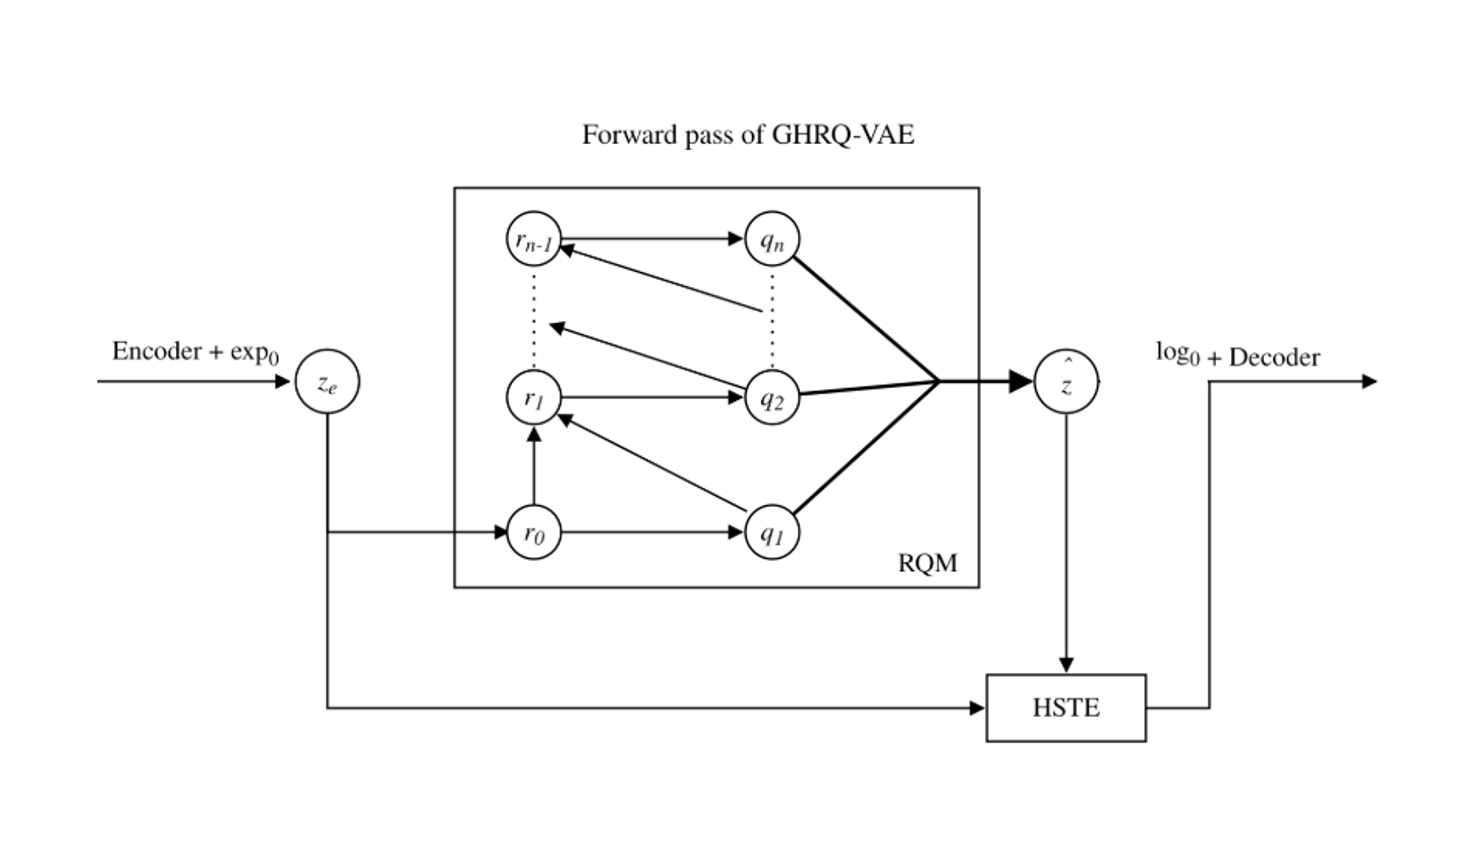
\includegraphics[width=\textwidth]{thesis/new_scheme.png}
    \caption{Forward pass of the GHRQ module. The encoder output $z_e$ is residual-quantized into coarse-to-fine codes $q_1,\dots,q_{n_q}$, which are recombined under the Hyperbolic Residual Aggregation order $\hat z = q_1\oplus_c(q_2\oplus_c(\cdots\oplus_c q_{n_q}))$ (Eq.~\ref{eq:hrq_residual}) to land on $z_e$ up to the unquantized tail. The block-level gradient routing of \S\ref{sec:blockste} sends a single discounted-HSTE gradient from $\hat z$ directly back to $z_e$, bypassing the intermediate codes and residuals. All the bacward passes through the RQM are blocked, except for the coarsest commitment path from $q_1$ to $z_e$, which is left intact to preserve codebook optimizability.}
    \label{fig:ghrq_scheme}
\end{figure}

\chapter{Experimental Setup}
\label{chap:expsetup}

The methodology introduced in Chapter~\ref{chap:methods} provides a geometry- and architecture-agnostic framework for residual quantization on the Poincar\'e ball. To evaluate this formulation against Euclidean and naive hyperbolic baselines, we test the quantizer across four tasks: WordNet hypernymy prediction, generative sequential recommendation (Amazon Reviews), image reconstruction and generation (MNIST, CIFAR-100), and neural audio coding (LibriTTS at 24\,kHz). These tasks span both the shallow regime ($n_q=4$), typical of prior hyperbolic residual quantization studies, and the deep regime ($n_q=12$), where the numerical instabilities discussed in \S\ref{sec:fail2} become pronounced.

Across all experiments, the quantizer geometry and gradient routing serve as the sole independent variables. The encoder, decoder, optimizer, data pipeline, and evaluation protocols remain strictly fixed within each task. We evaluate three distinct quantizer configurations: a Euclidean residual vector quantization baseline, a naive hyperbolic quantizer (\S\ref{sec:firewall}), and the proposed GHRQ-VAE (\S\ref{sec:blockste}). We detail configurations, tasks, architectures, hyperparameters, and metrics in \S\ref{sec:configs}--\S\ref{sec:metrics}. All experiments are conducted on a SLURM-managed HPC cluster utilizing NVIDIA A100 and H100 GPUs. The source code is publicly available.\footnote{\url{https://github.com/Sland0r/HyperbolicVQ}}

\section{Baselines}
\label{sec:configs}

The experimental design isolates the impact of geometry and gradient routing by evaluating three quantizer configurations with identical capacity. For any given task, all configurations share the number of residual stages ($n_q$), codebook sizes, and encoder/decoder architectures.

\paragraph{Euclidean (baseline).} This configuration employs standard residual vector quantization ($c=0$) with an identity straight-through estimator and an additive residual recursion ($r_i = r_{i-1}-q_i$, $\hat z=\sum_i q_i$) as described in \S\ref{sec:bg_rvq}. It serves as the primary baseline.

\paragraph{Naive hyperbolic.} This directly adapts prior hyperbolic residual quantization methods~\cite{hrqvae} ($c=1$), as detailed in \S\ref{sec:firewall}. While codebooks reside on the Poincar\'e ball and assignments utilize squared geodesic distance, the estimator retains the Euclidean identity straight-through estimator and employs M\"obius addition (Eq.~\ref{eq:prev_residual}). Consequently, it is subject to the geometrical inaccuracies (\S\ref{sec:fail1}) and residual leakage (\S\ref{sec:fail2}) identified in the backward-pass analysis.

\paragraph{Diagnostic gradient-routing variants.} Beyond the two primary configurations, \S\ref{sec:rq_signal} introduces two diagnostic variants that manipulate only the backward gradient routing to probe whether the per-stage reconstruction signal leaked by the naive baseline (\S\ref{sec:fail2}, Eq.~\ref{eq:stack}) is useful. The first, \emph{naive hyperbolic + sg}, detaches the residual after each M\"obius update ($r_i\leftarrow\operatorname{sg}[r_i]$), severing gradient paths from deeper codes to isolate the leaked contribution. The second, \emph{GHRQ-VAE + RQ signal}, retains GHRQ-VAE's block-level hop but reinstates the per-stage reconstruction gradients, testing whether the leaked signal can be folded back into the geometry-aware estimator.

\section{Tasks and Datasets}
\label{sec:tasks}

\subsection{WordNet Hypernymy Prediction}
\label{sec:tasks_nlp}
This task embeds the WordNet noun hierarchy~\cite{nickel2017poincare}, consisting of $82{,}115$ noun synsets and their associated hypernymy edges extracted via NLTK. The encoder is optimized via a contrastive InfoNCE objective, contrasting positive hypernymy edges against $50$ sampled negatives. The transitive closure is employed to prevent the sampling of true ancestors as negatives. Evaluation utilizes the \emph{closure} split, which requires composing transitive relations to reconstruct held-out edges. For context, a no-model graph-composition baseline achieves approximately $80\%$ recall@10 on this split, while a global-popularity baseline attains approximately $41\%$.

\subsection{Generative Sequential Recommendation}
\label{sec:tasks_rec}
Following the semantic-ID paradigm~\cite{tiger}, this task maps individual items to a tuple of discrete codes via residual quantization. Subsequently, a sequence model predicts the codes of the next item based on user interaction history. We utilize the Beauty category of the Amazon Reviews 2014 corpus under a standard leave-one-out evaluation protocol. Items are initially encoded into $768$-dimensional sentence embeddings using a pretrained MPNet sentence-transformer. These frozen embeddings serve as the input for quantization. Consistent with standard practice, a uniqueness tie-break token is appended to disambiguate items that map to identical code tuples.

\subsection{Image Reconstruction and Generation}
\label{sec:tasks_image}
The image domain evaluation utilizes MNIST ($28\times28$ grayscale, $60{,}000$ training and $10{,}000$ test images) and CIFAR-100 ($32\times32$ RGB, $50{,}000$ training and $10{,}000$ test images). CIFAR-100 provides a structured two-level label hierarchy, comprising $100$ fine classes organized into $20$ coarse superclasses. This structure evaluates unsupervised taxonomy recovery within the quantized latent space (\S\ref{sec:metrics}). Pixel values are normalized to $[-1,1]$, and no data augmentation is applied to strictly isolate the quantizer's effect.

\subsection{Neural Audio Coding}
\label{sec:tasks_audio}
The audio evaluation employs a SoundStream-style neural codec~\cite{soundstream,encodec} trained on the \texttt{train-clean-100} subset of LibriTTS at a $24$\,kHz sample rate. This setting represents the deepest evaluated stack, featuring $n_q=12$ residual quantizers with $1024$ codes per stage. This configuration subjects the intermediate residuals to severe boundary proximity, testing the depth-related pathologies identified in \S\ref{sec:fail2}. Due to the divergence of conformal factors near the boundary (Eq.~\ref{eq:hste_backward}), the hyperbolic codec necessitates explicit encoder stabilization, specifically an encoder-scale control and quantizer-depth dropout~\cite{soundstream}. Results are reported for a codebook dimension of $64$ over a $10$-epoch training budget.

The encoder-scale control addresses the tendency of high-dimensional encoder outputs (tangent norm $\sim\!\sqrt{d}$) to map directly to the boundary via the exponential map, which saturates geodesic distance and causes vanishing gradients. We implement an auto-calibrated global multiplier on the encoder tangent vectors, targeting a median residual radius of $0.5$. This scale is maintained via an exponential moving average ($s \leftarrow 0.99s + 0.01s_{\text{batch}}$), actively preventing the drift of deep residuals toward the boundary over the course of training.

\section{Model Architectures}
\label{sec:models}

\paragraph{WordNet Hypernymy Prediction.} A fully-connected embedding network maps synsets to a $16$-dimensional vector, which is projected onto the manifold and quantized ($n_q=4$, $128$ codes). Recall@10 is evaluated using an autoregressive seq2seq model with beam search, predicting hypernym code tuples, trained for $10$ epochs on the frozen representations.

\paragraph{Generative Sequential Recommendation.} The quantizer is instantiated as an RQ-VAE~\cite{lee2022rqvae,hrqvae} featuring a $768\!\to\!512\!\to\!32$ MLP encoder and symmetric decoder ($n_q=4$, $128$ codes). The downstream recommender is an encoder-decoder Transformer (dimension $384$, $6$ layers, $6$ heads, feed-forward dimension $1024$, dropout $0.1$), generating semantic IDs autoregressively via beam search ($50$ beams, history length $20$).

\paragraph{Image Reconstruction and Generation.} A convolutional VQ-VAE~\cite{vqvae} is employed. The encoder comprises strided $2$-D convolutions ($\text{in}\to32\to64\to128\to D$ channels) yielding a spatial downsampling factor of four, followed by the residual quantizer ($n_q=4$, with latent dimension $D=8$ and $128$ codes per stage for MNIST, and $D=16$ and $512$ codes per stage for CIFAR-100). The decoder utilizes symmetric transposed convolutions. For generative modeling, an RQ-Transformer prior~\cite{lee2022rqvae} (spatial and depth transformers, $4$ layers each, $8$ heads, $256$ dimensions) is trained over the frozen quantizer, from which $10{,}000$ samples are drawn.

\paragraph{Neural Audio Coding.} We build on the AcademiCodec implementation~\cite{academicodec}, utilizing a SEANet convolutional architecture~\cite{soundstream,encodec} paired with a $12$-stage residual quantizer ($1024$ codes per stage). Training employs an adversarial objective incorporating multi-scale STFT, multi-period, and multi-scale waveform discriminators, alongside reconstruction and feature-matching losses. Adversarial training commences after $500$ steps.

\section{Training Hyperparameters}
\label{sec:hparams}

Base parameters are generally optimized using AdamW, while manifold parameters (codebooks) utilize Riemannian Adam \cite{geoopt}. Curvature is uniformly set to $c=1$ for hyperbolic models.

The per-task training budgets, learning rates, and commitment weights are as follows. The image VQ-VAE trains for $50$ epochs with a base learning rate of $3\times10^{-4}$ (codebooks $10^{-4}$) and a commitment weight of $0.25$. The WordNet encoder trains for $50$ epochs with Riemannian SGD at a learning rate of $1.0$ and a commitment weight of $1.0$, after which the downstream seq2seq recall model trains for $10$ epochs. The recommendation RQ-VAE trains for $5000$ epochs at a learning rate of $10^{-4}$, weighting reconstruction by $1000$ and commitment by $0.01$, and its downstream recommender trains for $100$ epochs at the same learning rate. The audio codec trains for $10$ epochs with a base learning rate of $3\times10^{-4}$ (codebooks $10^{-4}$) and a commitment weight of $0.25$.

\section{Evaluation Metrics}
\label{sec:metrics}

Each configuration is evaluated on task-specific performance criteria and, where applicable, on the structural hierarchy of the learned latent space, to distinguish reconstruction fidelity from hierarchical organization.

\paragraph{WordNet Hypernymy Prediction.} Performance is evaluated via Recall@10 for hypernymy reconstruction on the closure split using beam search. Latent representation quality is further analyzed through code-tuple uniqueness and intra-cluster semantic coherence. Coherence is quantified using WordNet path similarity (inverse graph distance in the taxonomy), Wu--Palmer tree similarity (relatedness from the depth of the lowest common ancestor), and cosine similarity of GloVe embeddings.

\paragraph{Generative Sequential Recommendation.} Sequential recommendation efficacy is measured via top-$k$ ranking on held-out items, reporting Recall@5/10 and NDCG@5/10. The pre-deduplication uniqueness ratio of generated semantic IDs is reported as a diagnostic measure of codebook utilization.

\paragraph{Image Reconstruction and Generation.} Reconstruction fidelity is measured by the optimal validation mean squared error. Generative modeling performance is evaluated using Fr\'echet Inception Distance (FID) and Inception Score (IS), computed on $10{,}000$ samples. Hierarchy recovery on CIFAR-100 is assessed by analyzing the mean code embeddings of the $100$ fine classes. We report, for an agglomerative clustering into $20$ groups compared against the ground-truth superclasses, the Adjusted Rand Index (ARI, chance-corrected agreement of cluster assignments), Normalized Mutual Information (NMI, shared information between clustering and labels), and purity (the fraction of points lying in their cluster's majority class).

\paragraph{Neural Audio Coding.} The primary evaluation metric is the optimal validation reconstruction loss. Perceptual rate-distortion is evaluated using PESQ (perceptual speech-quality score), STOI (correlation of speech envelopes), and SI-SDR (scale-invariant signal-to-distortion ratio in dB) metrics mapped against entropy-estimated bitrates.

\chapter{Results}
\label{chap:experiments}

We evaluate the three quantizer configurations of \S\ref{sec:configs} on the four tasks of \S\ref{sec:tasks}. Prior work~\cite{hrqvae} shows hyperbolic residual quantization improves performance on WordNet (\S\ref{sec:exp_nlp}) and sequential recommendation (\S\ref{sec:exp_rec}). On these tasks, we assess whether GHRQ-VAE outperforms the naive hyperbolic baseline. The remaining two tasks are image reconstruction and generation (\S\ref{sec:exp_image}) and neural audio coding (\S\ref{sec:exp_audio}). We present the first application of hyperbolic residual quantization to a convolutional image tokenizer and a deep ($n_q=12$) neural audio codec.

\section{WordNet Hypernymy Prediction}
\label{sec:exp_nlp}

The first of the two established-hierarchy tasks embeds the WordNet noun hypernymy graph (\S\ref{sec:tasks_nlp}), comparing the Euclidean baseline, the naive hyperbolic lift, and our GHRQ-VAE.

\begin{table}[h]
\centering
\caption{WordNet hypernymy reconstruction (Recall@10, closure split) across varying encoder dimensions ($d \in \{8, 16\}$) and per-stage codebook sizes ($b \in \{64, 128\}$). All other hyperparameters, including the number of quantization stages ($n_q=4$), are held constant. The hyperbolic formulations consistently outperform the Euclidean baseline across almost all capacity settings. The best performance for each configuration is highlighted in bold.}
\label{tab:nlp_grid}
\begin{tabular}{lcccc}
\hline
Configuration & $d8/b64$ & $d8/b128$ & $d16/b64$ & $d16/b128$ \\
\hline
Euclidean & $75.8$ & $75.4$ & $76.7$ & $75.9$ \\
Naive hyperbolic (old) & $\mathbf{88.2}$ & $62.3$ & $\mathbf{86.9}$ & $\mathbf{83.4}$ \\
GHRQ-VAE (ours) & $81.9$ & $\mathbf{78.7}$ & $83.8$ & $81.9$ \\
\hline
\end{tabular}
\end{table}

Table~\ref{tab:nlp_grid} reports the Recall@10 for hypernymy reconstruction across varying model capacities. While hyperbolic formulations consistently outperform the Euclidean baseline, the naive hyperbolic baseline is unstable. Although it achieves peak recall in specific configurations ($88.2\%$ at $d8/b64$), it collapses significantly in others ($62.3\%$ at $d8/b128$). Furthermore, its peak performance is artificially inflated by codebook collapse: Table~\ref{tab:nlp_repr} shows that the naive approach yields a low uniqueness ratio ($0.888$), assigning identical code sequences to disparate concepts, thereby reducing the target space for the reconstructor. Conversely, GHRQ-VAE provides a stable optimization profile and maintains high codebook utilization (uniqueness $0.967$). 

\begin{table}[h]
\centering
\caption{WordNet latent representation quality evaluated at the standard capacity setting ($d16/b128$) across all $82{,}115$ noun synsets. The uniqueness ratio denotes the proportion of distinct code sequences assigned per concept. The semantic similarity of concepts mapped to identical codes is evaluated using WordNet Path, Wu--Palmer tree similarity, and GloVe cosine similarity, with higher values indicating tighter clustering.}
\label{tab:nlp_repr}
\begin{tabular}{lcccc}
\hline
Configuration & uniq.\ ratio & path sim & wup sim & GloVe sim \\
\hline
Euclidean & $0.997$ & $0.123$ & $0.320$ & $0.336$ \\
Naive hyperbolic (old) & $0.888$ & $0.078$ & $0.242$ & $0.097$ \\
GHRQ-VAE (ours) & $0.967$ & $0.088$ & $0.262$ & $0.162$ \\
\hline
\end{tabular}
\end{table}

Crucially, as shown in Table~\ref{tab:nlp_repr}, GHRQ-VAE clusters the vocabulary into more semantically coherent groups, consistently outperforming the naive approach across Path, Wu--Palmer, and GloVe similarity metrics.

\section{Generative Sequential Recommendation}
\label{sec:exp_rec}

The recommendation task evaluates whether the improved hierarchical code space translates to downstream seq2seq generative recommendation (\S\ref{sec:tasks_rec}). As shown in Table~\ref{tab:rec_beauty}, both hyperbolic methods outperform the Euclidean baseline. 

\begin{table}[h]
\centering
\caption{Downstream recommendation performance on the Amazon Beauty dataset. We report the test-set ranking metrics and the pre-deduplication uniqueness ratio (as a proxy for codebook health). Results show the mean over 3 runs. GHRQ-VAE employs the block-level gradient routing, though its depth-stabilizing effect at this depth ($n_q=4$) is negligible compared to the uncorrected variant. The best values per column are highlighted in bold.}
\label{tab:rec_beauty}
\begin{tabular}{lccccc}
\hline
Configuration & uniq.\ ratio & R@5 & NDCG@5 & R@10 & NDCG@10 \\
\hline
Euclidean & $0.960$ & $0.0352$ & $0.0242$ & $0.0530$ & $0.0299$ \\
Naive hyperbolic (old) & $0.870$ & $0.0388$ & $0.0259$ & $\mathbf{0.0606}$ & $0.0329$ \\
GHRQ-VAE (ours) & $\mathbf{0.971}$ & $\mathbf{0.0393}$ & $\mathbf{0.0264}$ & $0.0604$ & $\mathbf{0.0332}$ \\
\hline
\end{tabular}
\end{table}

Crucially, GHRQ-VAE resolves the codebook collapse affecting the naive approach, increasing the uniqueness ratio from $0.870$ to $0.971$. This restored codebook health directly translates to superior recommendation quality, with GHRQ-VAE achieving the highest performance on the majority of ranking metrics. Given the shallow stack ($n_q=4$), the block-level gradient routing has a negligible impact here; the primary advantage of GHRQ-VAE in this setting is the restoration of codebook utilization.

Section \ref{sec:rq_signal} analyzes the utility of the per-stage reconstruction signal.

\section{Image Reconstruction and Generation}
\label{sec:exp_image}

The image domain provides a multi-faceted evaluation of the quantizer's capabilities by scoring the same trained codes across three distinct criteria: compression fidelity (reconstruction MSE), token quality for generative modeling (RQ-Transformer FID/IS), and unsupervised taxonomy discovery. The hierarchy discovery evaluation follows the clustering methodology of \S\ref{sec:metrics}, utilizing superclass labels that remain strictly unseen during training. Tables~\ref{tab:img_recon}--\ref{tab:img_gen} summarize the results across these three dimensions.

\begin{table}[h]
\centering
\caption{Image reconstruction performance. We report the best validation reconstruction loss ($\times10^{-3}$, mean over three random seeds). The Euclidean baseline achieves the lowest reconstruction error across both datasets.}
\label{tab:img_recon}
\begin{tabular}{lcc}
\hline
Configuration & MNIST & CIFAR-100 \\
\hline
Euclidean & $\mathbf{0.477}$ & $\mathbf{1.077}$ \\
Naive hyperbolic & $0.600$ & $1.280$ \\
GHRQ-VAE (ours) & $0.647$ & $1.360$ \\
\hline
\end{tabular}
\end{table}

\begin{table}[h]
\centering
\caption{Unsupervised superclass hierarchy recovery on CIFAR-100 (mean over three seeds). Superclass labels were excluded during training. GHRQ-VAE demonstrates superior global tree structure recovery across primary clustering metrics (ARI, NMI, and Purity).}
\label{tab:img_hier}
\begin{tabular}{lccc}
\hline
Configuration & ARI & NMI & purity \\
\hline
Euclidean & $0.048$ & $0.469$ & $0.327$ \\
Naive hyperbolic & $0.055$ & $0.481$ & $0.337$ \\
GHRQ-VAE (ours) & $\mathbf{0.087}$ & $\mathbf{0.515}$ & $\mathbf{0.370}$ \\
\hline
\end{tabular}
\end{table}

\begin{table}[h]
\centering
\caption{Image generation performance utilizing an autoregressive RQ-Transformer ($10{,}000$ samples, single seed). We report Fr\'echet Inception Distance (FID, lower is better) and Inception Score (IS, higher is better) in parentheses. Hyperbolic formulations outperform the Euclidean baseline on MNIST, whereas Euclidean quantization yields superior generation on CIFAR-100.}
\label{tab:img_gen}
\begin{tabular}{lcc}
\hline
Configuration & MNIST FID (IS) & CIFAR-100 FID (IS) \\
\hline
Euclidean & $20.36\ (2.069)$ & $\mathbf{94.67}\ (3.86)$ \\
Naive hyperbolic & $\mathbf{15.01}\ (2.105)$ & $101.84\ (3.51)$ \\
GHRQ-VAE (ours) & $16.78\ (2.068)$ & $98.23\ (3.80)$ \\
\hline
\end{tabular}
\end{table}

\paragraph{Image Reconstruction.}
The Euclidean baseline yields the lowest reconstruction error (Table~\ref{tab:img_recon}). Both hyperbolic configurations incur a $25$--$30\%$ relative MSE penalty, with GHRQ-VAE performing marginally behind the naive lift. This behavior is consistent with the theoretical analysis in \S\ref{sec:blockste}, which anticipates that the geometrically corrected estimator improves gradient transport and representation structure rather than optimizing raw continuous distortion. More broadly, the penalty reflects how hyperbolic curvature reallocates a fixed representational capacity away from raw signal reconstruction, a trade-off whose returns appear in the structural and generative criteria below.

\paragraph{Hierarchy Recovery.}
When assessing the structural organization of the code space (Table~\ref{tab:img_hier}), the performance ranking inverts. GHRQ-VAE improves global clustering metrics on CIFAR-100, increasing the Adjusted Rand Index (ARI) from the Euclidean baseline's $0.048$ to $0.087$ ($+80\%$). It similarly leads in Normalized Mutual Information (NMI) and Purity. These results align closely with the hyperbolic hypothesis: for datasets possessing a latent taxonomy, operating on a manifold with constant negative curvature facilitates the discovery and embedding of hierarchical relationships. The capacity surrendered at the reconstruction stage is thus recovered here as a more robust global taxonomy, confirming that structural organization and raw distortion behave as distinct, sometimes competing, objectives.

\paragraph{Image Generation.}
The generative modeling performance (Table~\ref{tab:img_gen}) is notably dataset-dependent. On MNIST, both hyperbolic configurations achieve superior FID scores compared to the Euclidean baseline, indicating that hyperbolic codes can serve as more effective autoregressive tokens despite their higher reconstruction error. Conversely, on CIFAR-100, the Euclidean baseline yields the best FID, with GHRQ-VAE acting as the strongest hyperbolic alternative. This dataset-dependence shows that the reallocated capacity also feeds generative token quality, but only in specific regimes: the same curvature that improves next-token predictability on MNIST does not transfer to the more complex CIFAR-100 distribution. Taken together, the three criteria—reconstruction fidelity, generative token quality, and hierarchical organization—therefore behave as distinct objectives governed by the underlying geometry of the latent space, with hyperbolic curvature trading raw signal fidelity for structural and, in places, generative gains.

\section{Neural Audio Coding}
\label{sec:exp_audio}

\paragraph{Experimental Setup.}
The neural audio coding task utilizes the deep configuration ($n_q=12$) to evaluate the scalability of the proposed block-level estimator under extended depth, specifically testing its robustness against the depth-induced gradient pathologies identified in \S\ref{sec:fail2}. 

\paragraph{Boundary Regularization.}
The hyperbolic codec requires the specific boundary controls detailed in \S\ref{sec:tasks_audio}. These include an encoder-scale boundary regularizer and uniform quantizer-depth dropout, both of which are required to prevent representation collapse across all hyperbolic configurations.

\paragraph{Perceptual Quality and Dimensionality.}
Table~\ref{tab:audio_rd} presents the perceptual rate--distortion metrics at the maximum quantization depth ($n_q=12$). The Euclidean baseline consistently yields the highest perceptual quality across all evaluated dimensionalities ($d \in \{8, 32, 64, 128, 512\}$), outperforming both the naive hyperbolic baseline and the GHRQ-VAE. While the hyperbolic configurations manage to prevent total objective reconstruction collapse, they only produce viable perceptual representations at specific low-to-mid dimensions (e.g., $d=32$ for GHRQ-VAE and $d=64$ for the naive baseline). At other dimensions, the hyperbolic models exhibit severe degradation in subjective quality metrics.

\paragraph{Rate--Distortion Scaling.}
The rate--distortion scaling behavior is further detailed in Figure~\ref{fig:audio_rd}, which illustrates performance across the depth sweep ($n_q\in\{1,2,4,8,12\}$). The Euclidean framework maintains a superior Pareto frontier relative to all hyperbolic configurations. Notably, across all methods, the rate--distortion curves plateau after the second quantization stage ($n_q=2$). This indicates that while deeper residual stages increase the empirical entropy rate, they fail to contribute improvements to the perceptual fidelity of the reconstructed audio.

% --- 10-epoch perceptual rate-distortion at full depth (n_q=12) ---
\begin{table}[H]
\centering
\caption{Perceptual rate--distortion performance at maximum quantization depth ($n_q=12$), evaluated on $100$ dev-clean utterances. We report PESQ-wb and STOI (higher is better) for each quantizer variant (Euclidean, naive hyperbolic, and GHRQ-VAE) across codebook dimensions. Underlined GHRQ entries mark the configurations where the GHRQ-VAE improves on the naive hyperbolic baseline, which holds for every dimension except $d{=}64$. The Euclidean baseline achieves the optimal perceptual quality across all tested dimensions. In contrast, hyperbolic configurations only maintain valid perceptual representations at restricted lower dimensions. At other dimensions, the hyperbolic models exhibit severe degradation in perceptual metrics despite maintaining non-collapsed objective reconstruction losses.}
\label{tab:audio_rd}
\begin{tabular}{lccc|ccc}
\hline
 & \multicolumn{3}{c|}{PESQ$\uparrow$} & \multicolumn{3}{c}{STOI$\uparrow$} \\
\cline{2-7}
dim & Euclidean & Naive & GHRQ (ours) & Euclidean & Naive & GHRQ (ours) \\
\hline
$8$   & $1.506$ & $1.192$ & $\underline{1.391}$ & $0.872$ & $0.793$ & $\underline{0.848}$ \\
$32$  & $1.665$ & $1.143$ & $\underline{1.448}$ & $0.889$ & $0.773$ & $\underline{0.854}$ \\
$64$  & $1.685$ & $1.369$ & $1.115$ & $0.890$ & $0.846$ & $0.752$ \\
$128$ & $1.654$ & $1.121$ & $\underline{1.269}$ & $0.893$ & $0.735$ & $\underline{0.814}$ \\
$512$ & $1.480$ & $1.087$ & $\underline{1.109}$ & $0.858$ & $0.697$ & $\underline{0.706}$ \\
\hline
\end{tabular}
\end{table}

\begin{figure}[H]
\centering
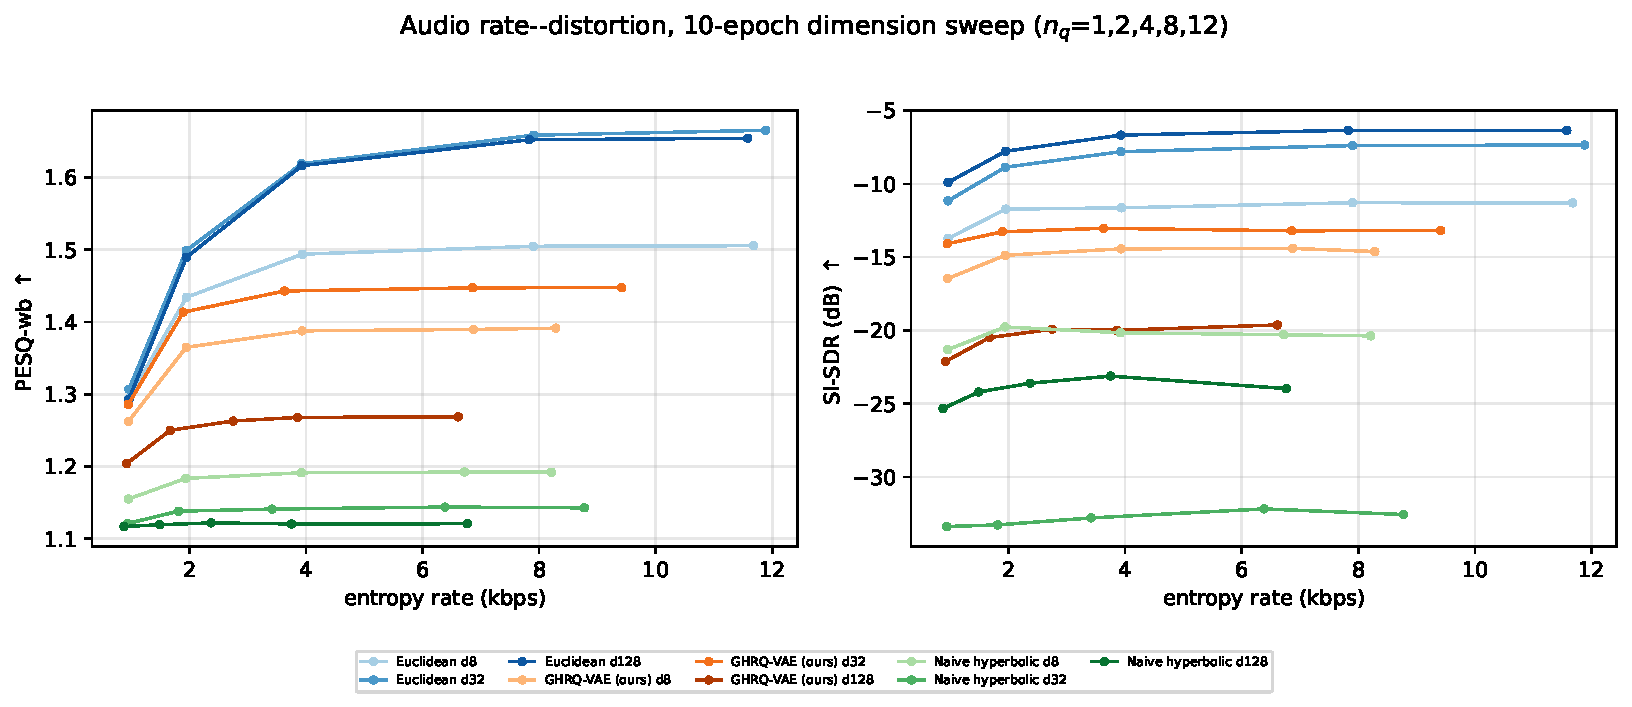
\includegraphics[width=\textwidth]{thesis/audio_rd_curves.pdf}
\caption{Rate--distortion performance across varying quantization depths ($n_q\in\{1,2,4,8,12\}$), plotted against the empirical entropy rate. Individual markers denote distinct operating points. The color indicates the quantizer variant (blue: Euclidean; orange: GHRQ-VAE; green: naive hyperbolic lift), while shading represents the codebook dimensionality ($d\in\{8,32,128\}$). Left panel: PESQ-wb metric. Right panel: SI-SDR metric. The Euclidean configurations consistently achieve superior perceptual quality relative to the hyperbolic variants across all tested bitrates. Among the hyperbolic methods, however, our GHRQ-VAE (orange) almost everywhere dominates the naive lift (green), attaining higher perceptual quality at matched entropy rate across nearly all operating points and dimensions. Furthermore, the performance curves plateau after $n_q=2$, indicating that subsequent residual quantization stages increase the empirical entropy rate without yielding proportional improvements in perceptual quality.}
\label{fig:audio_rd}
\end{figure}

\section{Residual Reconstruction Error Across Tasks}
\label{sec:exp_approx}

This section evaluates whether GHRQ-VAE enables the residual cascade to accurately reconstruct the encoder output on the Poincar\'e ball, overcoming the gyration drift of the naive baseline (Eq.~\ref{eq:prev_residual}). Reconstruction accuracy is quantified by the squared hyperbolic distance between the aggregated codes and the encoder output. Table~\ref{tab:approx} presents the mean validation reconstruction errors.

\begin{table}[H]
\centering
\caption{Mean validation reconstruction error on the Poincar\'e ball, measured as the squared hyperbolic distance between the reconstructed code aggregate and the encoder output. Lower values indicate greater reconstruction fidelity. The naive baseline employs the prior M\"obius transliteration, whereas the GHRQ-VAE utilizes the HRA ordering and gradient correction.}
\label{tab:approx}
\begin{tabular}{llcc}
\hline
Task & Cell & Naive hyperbolic & GHRQ-VAE (ours) \\
\hline
Image  & MNIST            & $0.00049$ & $<\!10^{-5}$ \\
Image  & CIFAR-100        & $0.00133$ & $<\!10^{-5}$ \\
Rec    & Beauty           & $44.79$   & $0.031$ \\
Audio  & $d8$, $10$ ep    & $0.403$   & $0.0016$ \\
Audio  & $d32$, $10$ ep   & $0.413$   & $0.0023$ \\
Audio  & $d64$, $10$ ep   & $0.805$   & $0.0021$ \\
Audio  & $d128$, $10$ ep  & $0.747$   & $0.0092$ \\
Audio  & $d512$, $10$ ep  & $57.77$   & $2.420$ \\
NLP    & $d16/b128$       & $14.4$ & $12.9$ \\
\hline
\end{tabular}
\end{table}

\paragraph{General Reconstruction Efficacy.}
The empirical results corroborate the theoretical predictions outlined in \S\ref{sec:newmethod}. The GHRQ-VAE learns to reconstruct the encoder representation on the manifold with high precision, yielding residual errors that converge near zero. This is particularly evident in the recommendation task, where our method achieves an error of $0.031$, compared to $44.79$ for the naive baseline. Similarly, across the audio dimension sweep ($d8$ through $d128$), the GHRQ formulation maintains a restricted error band of $0.0016$--$0.0092$. Under identical hyperparameters, the naive formulation produces errors ranging from $0.403$ to $0.805$. To verify that this reduction stems from the HRA telescoping property, we conduct ablation studies.

\paragraph{Impact of Curvature-Scaled Radius.}
The exactness of the telescoping property depends on the operating radius within the Poincar\'e ball. For the widest audio codebook ($d512$), the reconstruction error increases for both methods. This correlates with the perceptual collapse previously observed for this configuration (Table~\ref{tab:audio_rd}). The increased residual error functions as an on-ball indicator of codes distributed at a large curvature-scaled radius, rather than a fundamental failure of the HRA ordering. This reveals a limitation when scaling to high latent dimensions: extreme curvature-scaled radii make it difficult to maintain precise representations. As shown in \S\ref{sec:abl_components}, d-HSTE controls this radius growth. Consequently, configurations employing d-HSTE telescope more precisely than uncorrected variants.

\section{Is the Residual Quantization Signal Useful?}
\label{sec:rq_signal}

A recurring observation across the preceding experiments is that the naive hyperbolic lift, despite being geometrically inexact, is occasionally the stronger model: it attains the best shallow WordNet recall (Table~\ref{tab:nlp_grid}) and leads on recommendation R@10 (Table~\ref{tab:rec_beauty}). This violates the residual firewall of \S\ref{sec:fail2}: instead of returning a single clean gradient copy, the naive estimator leaks the accumulated per-stage reconstruction signal (Eq.~\ref{eq:stack}). This section asks whether that leaked signal is genuinely informative, and if it can be folded back into GHRQ-VAE. We answer this using the two diagnostic variants defined in \S\ref{sec:configs}: \emph{naive hyperbolic + sg} and \emph{GHRQ-VAE + RQ signal}.

\paragraph{The leak helps at shallow depth.}
On the shallow ($n_q=4$) WordNet model, keeping the leak is uniformly better across the trainable capacity region: in every cell of Table~\ref{tab:gc_leak} the naive model outperforms its gradient-corrected counterpart. The same direction holds on recommendation, where the plain naive lift stays competitive with the corrected block-hop variant and even leads on R@10 (Table~\ref{tab:rec_beauty}). These shallow stacks are precisely the regimes in which prior hyperbolic residual-quantization work reported strong results: when only a handful of short leak matrices are ever composed, the superposition is a low-variance, on-average-correct supervisory signal, geometrically inexact yet providing a correct directional signal.

\begin{table}[h]
\centering
\caption{WordNet Recall@10 (\%), shallow $n_q=4$: keeping the leaked residual gradient (naive hyperbolic) versus removing it, across the trainable $d{=}16$ capacity region.}
\label{tab:gc_leak}
\begin{tabular}{lccc}
\hline
Method & $d16/b64$ & $d16/b128$ & $d16/b256$ \\
\hline
Naive hyperbolic       & \textbf{86.9} & \textbf{83.4} & \textbf{81.7} \\
Naive hyperbolic + sg  & 83.5 & 82.3 & 80.5 \\
\hline
\end{tabular}
\end{table}

\paragraph{Reinstating the signal in GHRQ-VAE.}
We subsequently investigate whether this informative shallow signal can be combined with GHRQ-VAE's geometrically corrected block-level gradient: the \emph{GHRQ-VAE + RQ signal} configuration tests exactly this. Its behaviour is sharply task-dependent (Table~\ref{tab:rq_signal_hybrid}). On WordNet the reinstated signal is constructive, lifting recall over GHRQ-VAE in every capacity cell, most strongly in the higher-capacity regimes ($+3.1$ at $d16/b128$). On recommendation the same addition is mildly harmful, with the ranking metrics regressing back toward the Euclidean baseline. A numerically stable mechanism to combine it with the block-level estimator at depth remains open. We however exclude it from the primary GHRQ-VAE formulation, retaining the single block-level hop for its robustness.

\begin{table}[h]
\centering
\caption{Effect of reinstating the per-stage residual signal in GHRQ-VAE ($n_q=4$). Left: WordNet Recall@10 (\%) across the capacity grid. Right: Amazon Beauty ranking. Bold marks the better of the two configurations per column.}
\label{tab:rq_signal_hybrid}
\begin{tabular}{l|cccc|cc}
\hline
 & \multicolumn{4}{c|}{WordNet Recall@10 (\%)} & \multicolumn{2}{c}{Beauty} \\
Configuration & $d8/b64$ & $d8/b128$ & $d16/b64$ & $d16/b128$ & R@10 & NDCG@10 \\
\hline
GHRQ-VAE (ours)        & $81.9$ & $78.7$ & $83.8$ & $81.9$ & $\mathbf{0.0604}$ & $\mathbf{0.0332}$ \\
GHRQ-VAE + RQ signal   & $\mathbf{84.6}$ & $\mathbf{81.0}$ & $\mathbf{84.6}$ & $\mathbf{85.0}$ & $0.0579$ & $0.0316$ \\
\hline
\end{tabular}
\end{table}

\chapter{Ablations}
\label{ch:ablation}

\label{sec:abl_components}

GHRQ-VAE combines two modifications to the naive baseline: HRA (\S\ref{sec:residagg}) and d-HSTE (\S\ref{sec:hste}). To isolate their contributions we remove one component at a time while holding all other hyperparameters fixed:
\begin{itemize}
  \item \textbf{HRA, no d-HSTE:} the HRA forward ordering with the gradient estimator reverted to the Identity STE, testing the forward modification in isolation.
  \item \textbf{d-HSTE, no HRA:} the block-level d-HSTE applied over the naive M\"obius aggregation of \S\ref{sec:hrq}, testing the backward modification in isolation.
\end{itemize}
All ablations use the same configurations of the original experiments. Downstream task quality (recommendation ranking, image reconstruction MSE) is statistically unchanged across both ablation configurations and the full model in every domain, so we restrict attention to the two metrics that separate the components: the forward residual error and the hierarchical structure of the learned codes (\S\ref{sec:abl_hierarchy}).

\section{Effect on the Residual Error}

Table~\ref{tab:abl_residual} collects the on-ball residual error across the WordNet, recommendation, and image tasks.

\begin{table}[h]
\centering
\caption{Effect of the component ablation on the on-ball residual error ($n_q=4$). We report the mean validation squared hyperbolic distance between the recomposed codes and the encoder output; image columns are scaled by $10^{-3}$. The full GHRQ-VAE values correspond to those in Table~\ref{tab:approx}. Bold indicates the best result per column.}
\label{tab:abl_residual}
\begin{tabular}{cc|cccc}
\hline
HRA & BS d-HSTE & WordNet & Rec.\ (Beauty) & MNIST ($\times10^{-3}$) & CIFAR ($\times10^{-3}$) \\
\hline
\checkmark & $\times$     & $\mathbf{10.3}$ & $5.49$          & $0.01$          & $0.03$ \\
$\times$   & \checkmark   & $30.4$          & $0.12$          & $0.02$          & $0.05$ \\
\checkmark & \checkmark   & $12.9$          & $\mathbf{0.04}$ & $\mathbf{0.00}$ & $\mathbf{0.00}$ \\
\hline
\end{tabular}
\end{table}

HRA is not, on its own, what minimizes this error. The HRA ordering guarantees telescoping algebraically (\S\ref{sec:residagg}), yet the configuration that retains it without the corrected gradient is the least faithful on recommendation ($5.49$ against a baseline of $0.04$). Symmetrically, removing HRA is harmless on recommendation and images but inflates the WordNet error to $30.4$. While HRA alone is sufficient to minimize the error on WordNet, neither component is sufficient on its own across all domains: only the full model achieves uniformly low error. The algebraic guarantee of HRA holds only at the radii actually visited during training, and those radii are set by the encoder that d-HSTE trains more precisely; conversely, the corrected gradient recomposes faithfully only when the RQ's forward pass is ordered to telescope. Each component typically supplies the precondition the other requires.

\section{Effect on Hierarchical Representations}
\label{sec:abl_hierarchy}

\begin{table}[h]
\centering
\caption{Hierarchy recovery metrics for the CIFAR-100 superclasses under the component ablation ($n_q=4$, $b512$). We report the mean over seeds $42/43/44$ (higher is better); superclass labels are withheld during training. Bold indicates the best result per column.}
\label{tab:abl_img_hier}
\begin{tabular}{cc|ccc}
\hline
HRA & BS d-HSTE & ARI & NMI & purity \\
\hline
\checkmark & $\times$     & $0.055$          & $0.485$          & $0.340$ \\
$\times$   & \checkmark   & $\mathbf{0.089}$ & $0.511$          & $\mathbf{0.370}$ \\
\checkmark & \checkmark   & $0.087$          & $\mathbf{0.515}$ & $\mathbf{0.370}$ \\
\hline
\end{tabular}
\end{table}

The difference is sharpest in the unsupervised recovery of the CIFAR-100 superclass taxonomy (Table~\ref{tab:abl_img_hier}). Removing HRA leaves hierarchy recovery essentially unchanged: it matches the full model on every metric (ARI $0.089$ vs.\ $0.087$, purity $0.370$ vs.\ $0.370$). Removing d-HSTE degrades it across the board: it falls to ARI $0.055$ and purity $0.340$. The component responsible for representing hierarchy is thus the hyperbolic gradient estimator, and not the forward ordering. d-HSTE trains an encoder whose geometry arranges semantically related inputs coarse-to-fine on the ball, and this structure survives the removal of HRA but not the removal of the corrected gradient.

The WordNet task qualifies this conclusion in one respect (Table~\ref{tab:abl_nlp}). There, d-HSTE is necessary for codebook health rather than merely beneficial: in the experiment with no HRA, codebook diversity is preserved on recommendation (uniqueness $0.975$) and images, but on WordNet the same configuration collapses, mapping over $46{,}000$ of the $82{,}115$ synsets to shared code sequences (uniqueness $0.430$) and shedding $4.5$ points of Recall@10 (from $81.9$ to $77.4$). The interaction with HRA is thus task-dependent, but the direction is consistent: wherever hierarchical structure is recovered, it is the hyperbolic gradient estimator that recovers it.

\begin{table}[h]
\centering
\caption{Component ablation on the WordNet hypernymy task ($n_q=4$, $d16/b128$, closure split, single run). We report Recall@10 (\%) and the uniqueness ratio (the proportion of the $82{,}115$ noun synsets assigned a distinct code sequence; higher is better). Bold indicates the best result per column.}
\label{tab:abl_nlp}
\begin{tabular}{cc|cc}
\hline
HRA & BS d-HSTE & Recall@10 & Uniq.\ \\
\hline
\checkmark & $\times$     & $78.1$          & $\mathbf{0.968}$ \\
$\times$   & \checkmark   & $77.4$          & $0.430$ \\
\checkmark & \checkmark   & $\mathbf{81.9}$ & $0.967$ \\
\hline
\end{tabular}
\end{table}

\chapter{Conclusions}

This thesis reformulated residual quantization on the Poincar\'e ball as an intrinsic geometric operation. The proposed framework, GHRQ-VAE, introduces two modifications to the naive hyperbolic lift: Hyperbolic Residual Aggregation (HRA) to restore forward telescoping, and a block-level gradient routing (built on a discounted Hyperbolic Straight-Through Estimator (d-HSTE))  to route geometrically consistent, depth-independent gradients to the encoder. At zero curvature, the formulation strictly recovers standard Euclidean residual vector quantization.

Our evaluation across four domains highlights several key findings. First, hyperbolic curvature demonstrably aids hierarchical representation; while Euclidean models excel at raw reconstruction and remain competitive or better on several practical ranking metrics, the curved latent space naturally organizes hierarchical structure, yielding substantial gains in unsupervised CIFAR-100 superclass recovery and in WordNet hypernymy reconstruction (with better semantic clustering than the naive approach). Second, GHRQ-VAE offers a highly robust alternative to the naive lift, which frequently suffers from instability and codebook collapse. By maintaining codebook health, GHRQ-VAE achieves stable performance across varying capacities, with its advantages widening as the residual cascade deepens. Third, the proposed geometric corrections successfully align the residual codes with the encoder representation on the manifold. However, our results refute the hypothesis that hyperbolic geometry provides a superior pure compressor: Euclidean baselines consistently achieve lower reconstruction errors and better perceptual quality on raw distortion tasks. The principal advantage of GHRQ-VAE therefore lies in stable hierarchical structuring rather than pure signal fidelity.

Ablation studies further isolate the effects of the proposed components. Notably, minimizing the on-ball residual error across all domains requires both features: while HRA alone is sufficient for WordNet, HRA and d-HSTE effects generally compound. Furthermore, the block-level gradient routing combined with the corrected d-HSTE gradient emerges as the primary catalyst for capturing hierarchical representations.

A significant limitation of this work concerns the integration of distinct gradient signals. We proved that both the naive per-stage gradient and our block-level gradient carry informative and potentially complementary signals, with the former aiding shallow architectures and the latter stabilizing deeper ones. However, we did not thoroughly investigate how to efficiently combine these signals. Another fundamental limitation is the difficulty of scaling hyperbolic representations to high latent dimensions, where extreme curvature-scaled radii cause perceptual collapse and inflated residual errors. Finally, while we found that hyperbolic codes can serve as better autoregressive generative tokens on certain datasets like MNIST, recent state-of-the-art generation increasingly relies on diffusion and flow-matching models \cite{resgen}, so future work should evaluate hyperbolic tokenizers within these continuous paradigms. Developing a numerically stable mechanism to leverage both gradients simultaneously remains a critical avenue for future work, alongside evaluating GHRQ-VAE within large-scale modern tokenizers.

\appendix
%\chapter{Optional appendix}
\chapter{Method Motivation Analysis}
\section{Forward failure: non-telescoping residual cascade}
\label{sec:hrq}
In Hyperbolic VQ the Euclidean distance used to match the continuous vector to the codebook centroids is replaced by the squared hyperbolic distance. Given a vector $x \in \mathbb{D}_c^D$ and a codebook $C \subset \mathbb{D}_c^D$, the nearest-neighbour assignment is
\begin{equation}
    q(x) = c_k, \quad \text{where } k = \operatorname{argmin}_j d_{\mathbb{D}_c}^2(x, c_j),
\end{equation}
so that assignment strictly follows the geodesics of the manifold. Lifting the residual recursion of Eq.~\ref{eq:bg_rvq_residual} to the manifold then appears, at first sight, to be a matter of transliteration: replace Euclidean subtraction with M\"obius subtraction and Euclidean summation with M\"obius addition while preserving the order of operations. This is exactly the convention adopted by the naive approach. Writing $r_0 = z_e$ for the (projected) encoder output, stage $i$ selects $q_i = q(r_{i-1})$ and forms the next residual by \emph{right} M\"obius subtraction, while the output reaggregates the codewords by left-associated M\"obius addition in coarse-to-fine order:
\begin{equation}
    \label{eq:prev_residual}
    r_i = r_{i-1}\ominus_c q_i = r_{i-1}\oplus_c(-q_i),
    \qquad
    \hat z = \big(\cdots(q_1\oplus_c q_2)\oplus_c\cdots\big)\oplus_c q_{N} .
\end{equation}
These replace the Euclidean $r_i = r_{i-1}-q_i$ and $\hat z=\sum_i q_i$ of \S\ref{sec:bg_rvq} and keep every intermediate quantity on the ball.

\paragraph{The residual mismatch.} This transliteration is faithful in Euclidean space but breaks on the ball. The purpose of the residual is to track the portion of the encoder point not yet captured by the running reconstruction $\hat z_i = \big(\cdots(q_1\oplus_c q_2)\cdots\big)\oplus_c q_i$ formed from the first $i$ codes; the genuine remaining error is the \emph{true residual}
\begin{equation}
    \label{eq:true_residual}
    R_i^{\text{true}} := (-\hat z_i)\oplus_c z_e,
    \qquad\text{so that}\qquad
    \hat z_i \oplus_c R_i^{\text{true}} = z_e .
\end{equation}
In Euclidean Residual Vector Quantization the recursively tracked residual coincides with it, $r_i = z_e - \sum_{j\le i} q_j = R_i^{\text{true}}$, because addition is commutative and associative; the decomposition then telescopes exactly and $\hat z + r_{N} = z_e$. On the Poincar\'e ball neither property holds: right M\"obius subtraction is \emph{not} inverted by left-associated M\"obius addition, so the tracked residual $r_i$ of Eq.~\ref{eq:prev_residual} departs from the true residual $R_i^{\text{true}}$ of Eq.~\ref{eq:true_residual} by a gyration that the convention never accounts for, $r_i \neq R_i^{\text{true}}$. This mismatch is incurred at every stage and compounds with depth, so $\hat z\oplus_c r_{n_q}$ drifts away from $z_e$ even when every codeword is quantized without error. As a consequence, each codebook beyond the first is fitted to quantize a residual $r_i$ that no longer represents the actual reconstruction error $R_i^{\text{true}}$, and the deeper the stack the further the quantization target diverges from the quantity it is meant to encode.


\section{Forward repair: the HRA residual mismatch is a pure rotation}
\label{app:hra_proof}
Section~\ref{sec:residagg} repairs the forward cascade with the Hyperbolic Residual Aggregation (HRA) convention and states (Eq.~\ref{eq:hrq_norm}) that, under HRA, the tracked residual $r_i$ differs from the true residual $R_i^{\text{true}}$ only by a norm-preserving rotation. We supply the derivation here. Pulling the partial aggregate $\hat z_i=q_1\oplus_c(\cdots\oplus_c q_i)$ back out of $z_e$ through the reverse nesting, and repeatedly applying the gyration form of left cancellation,
\begin{equation}
    \label{eq:left_cancel_gyr}
    -(a\oplus_c b)\oplus_c(a\oplus_c c)=\operatorname{gyr}[a,b]\big((-b)\oplus_c c\big),
\end{equation}
relates the true and tracked residuals by a composition of gyrations,
\begin{equation}
    \label{eq:hrq_gyration}
    R_i^{\text{true}} = \Gamma_i\, r_i,
    \qquad
    \Gamma_i = \operatorname{gyr}\!\big[q_1,\;q_2\oplus_c\cdots\oplus_c q_i\big]\;\cdots\;\operatorname{gyr}\!\big[q_{i-1},\,q_i\big].
\end{equation}
Each factor is a gyration, hence (Eq.~\ref{eq:bg_gyration}) a norm-preserving rotation of the ball about the origin; their composition $\Gamma_i$ is therefore itself such a rotation, which rotates the \emph{direction} of the residual while adding \emph{zero} magnitude error. This establishes the norm equality $\|R_i^{\text{true}}\| = \|r_i\|$ of Eq.~\ref{eq:hrq_norm}: the tracked residual carries exactly the magnitude of the true reconstruction error at every depth, in sharp contrast with the naive convention of \S\ref{sec:hrq}, whose mismatch is not a rotation but a genuine drift that corrupts the residual magnitude and compounds with depth.


\section{Backward failures: distorted and cumulative gradient}
\label{sec:firewall}

\subsection{Failure 1: the copied gradient is not geometrically accurate}
\label{sec:fail1}
The naive hyperbolic lift breaks the \emph{backward} pass in two independent ways, and the first is present already in a \emph{single} quantization step, before any stages are stacked. Because the nearest-neighbour assignment $q=q(z_e)$ is non-differentiable, the lift keeps the Identity Straight-Through Estimator (Eq.~\ref{eq:bg_ste}): its forward value $z_e+\operatorname{sg}[q-z_e]=q$ has identity Jacobian, so the decoder's gradient $g_q:=\partial L/\partial q$ is passed to the encoder verbatim, $\partial L/\partial z_e=g_q$. In flat space this copy is exact; on the ball it is not even type-correct. The gradient $g_q$ is a tangent vector \emph{at the code}, $g_q\in T_q\mathbb{D}_c^D$, whereas the encoder update must live \emph{at the encoder point}, in $T_{z_e}\mathbb{D}_c^D$: two distinct tangent spaces carrying distinct conformal factors ($\lambda^c_q\neq\lambda^c_{z_e}$ in general). The faithful transfer between them is not the identity but the parallel transport $P^c_{q\to z_e}$ along the connecting geodesic (Eq.~\ref{eq:bg_pt}), bracketed by the metric (de)conversions of Eq.~\ref{eq:bg_riemgrad}; carried across this way, $g_q$ is rescaled by $\lambda^c_{z_e}/\lambda^c_q$ and rotated by $\operatorname{gyr}[z_e,-q]$:
\begin{equation}
    \label{eq:failure1}
    \underbrace{\frac{\partial L}{\partial z_e} = g_q}_{\text{identity Straight-Through Estimator copy}}
    \qquad\neq\qquad
    \underbrace{\frac{\lambda^c_{z_e}}{\lambda^c_q}\,\operatorname{gyr}[z_e,-q]\,g_q}_{\text{geometrically correct}} .
\end{equation}
The identity copy drops both corrections at once: the missing ratio $\lambda^c_{z_e}/\lambda^c_q$ corrupts the gradient's \emph{magnitude}, and, more importantly, the missing gyration corrupts its \emph{direction}. The encoder is pulled along a vector that is not the geodesic image of the decoder gradient, and this happens at all depths in the naive approach.

\subsection{Failure 2: the firewall leaks, so gradients accumulate}
\label{sec:fail2}
The second failure is structural and subtler than the single-step distortion above, so we first set up the residual recursion and the Euclidean gradient routing it ought to preserve, then show precisely how the naive lift breaks it.

\paragraph{The Residual Quantized Variational Autoencoders objective.}
Writing $r_{i-1}$ for the residual entering stage $i$ (with $r_0=z_e$) and $q_i$ for the code it selects, the model minimises
\begin{equation}
    \label{eq:rqvae_loss}
    \mathcal{L} = \underbrace{\lVert x - \hat x\rVert_2^2}_{\text{reconstruction}}
    \;+\; \sum_{i=1}^{n_q}\Big(
    \underbrace{d\big(\operatorname{sg}[r_{i-1}],\, q_i\big)^2}_{\text{codebook}}
    \;+\; \beta\,\underbrace{d\big(r_{i-1},\, \operatorname{sg}[q_i]\big)^2}_{\text{commitment}}
    \Big),
\end{equation}
where $\hat x = G(\hat z)$ is decoded from the aggregate code $\hat z = \sum_i q_i$, $\beta$ weights the commitment term, and $d(\cdot,\cdot)$ is a distance on the latent space: the Euclidean choice $d_{\mathbb{R}^D}(a,b)=\lVert a-b\rVert_2$ recovers the standard Residual Quantized Variational Autoencoders loss, while the geodesic distance of Eq.~\ref{eq:bg_distance} gives its hyperbolic counterpart. The reconstruction term reaches the encoder only through the chain of straight-through estimators; the per-stage codebook and commitment terms are the auxiliaries that train the dictionary and tie the encoder to it. Their stop-gradients separate their roles exactly: the codebook term, holding the residual fixed, moves \emph{only the codes}, whereas the commitment term, holding the code fixed, injects its gradient \emph{into the residual} $r_{i-1}$  (and hence back to the encoder). On the Poincar\'e ball $d$ is the geodesic distance and the residual subtraction and code sum become their M\"obius analogues (\S\ref{sec:residagg}), but these roles are unchanged.

\begin{figure}[t]
    \centering
    
\includegraphics[width=\textwidth]{thesis/scheme.png}
    \caption{Forward pass of the hyperbolic Residual Quantized Variational Autoencoders. The encoder $E$ produces a tangent vector that is mapped onto the Poincar\'e ball by $\exp_0^c$ to give the encoder point $z_e$ (the initial residual $r_0$). Inside the residual quantization module (RQM), each stage quantizes the current residual $r_{i-1}$ to a code $q_i$ and forms the next residual by M\"obius subtraction; the codes are recomposed by the aggregation operator (Agg, function of the chosen codes) into $\hat z$, which is mapped back to the tangent space by $\log_0^c$ and decoded by $G$. It is possible to reconstruct the gradient flow by following the arrows in reverse: the reconstruction gradient starts from the decoder and the commitment gradient is injected from each residual.}
    \label{fig:rqvae_schematic}
\end{figure}

\paragraph{The gradient flow.}
Failure~2 is exposed only by following the path the reconstruction signal actually takes back to the encoder. Figure~\ref{fig:rqvae_schematic} fixes the notation for the forward pass and shows that, with the identity Straight-Through Estimator in place, this signal can return to the encoder only through the residual branch traced below; the forward value $z_e+\operatorname{sg}[q(z_e)-z_e]=q(z_e)$ keeps every intermediate quantity on a codebook entry and never leaves the ball. To locate the leak we first ask why the flat case functions correctly, since the hyperbolic pathology reads cleanest as the breakdown of exactly that mechanism.

\paragraph{The Euclidean firewall.}
Two signals travel back toward the encoder: the reconstruction gradient, routed through the codes and the residual branch, and the commitment gradient, injected at each residual $r_{i-1}$. The residual branch governs both. Combining the Straight-Through Estimator Jacobian $\partial q_i/\partial r_{i-1}=I$ (Eq.~\ref{eq:bg_ste}) with the additive update $r_i = r_{i-1}-q_i$ (Eq.~\ref{eq:bg_rvq_residual}), the Jacobian of the residual branch is
\begin{equation}
    \label{eq:firewall}
    \frac{\partial r_i}{\partial r_{i-1}}
    = \frac{\partial (r_{i-1} - q_i)}{\partial r_{i-1}}
    = I - I = 0,
\end{equation}
so the residual branch transmits no gradient at all. We call this exact cancellation the residual gradient \emph{firewall}, and it filters both signals at once. The decoder produces a single gradient $g := \partial L_{\text{rec}}/\partial\hat z$ at the aggregate $\hat z=\sum_i q_i$; since $\hat z$ is the plain sum of the codes, every stage is handed the same $g$, yet the firewall cancels every residual-branch path except the shortest, whose empty product of residual Jacobians gives $\partial\hat z/\partial r_0 = I$. The encoder $r_0=z_e$ therefore receives \emph{exactly one} clean copy of $g$, independent of the depth $n_q$. The commitment terms are filtered identically: stage $i$'s term pulls $r_{i-1}$ toward $q_i$, but for $i>1$ the residual lies behind the firewall, so only the coarsest, $i=1$ term survives, while the codebook term by construction only ever trains the codes. This single depth-independent copy of the reconstruction gradient, together with the lone surviving commitment term, is what depth-stable training amounts to at the level of the gradient, and the concrete quantity we follow across the lift. The second failure below is precisely the loss of this routing once the residual subtraction is made hyperbolic.

\paragraph{The leak.}
This failure surfaces only once the steps are stacked. The Euclidean firewall rested on the exact cancellation $\partial r_i/\partial r_{i-1}=I-I=0$ (Eq.~\ref{eq:firewall}). Differentiating the M\"obius residual through both arguments of $\oplus_c$ gives, for a quantizer with straight-through Jacobian $J_i := \partial q_i/\partial r_{i-1}$,
\begin{equation}
    \label{eq:leak}
    \begin{aligned}
    A_i := \frac{\partial r_i}{\partial r_{i-1}}
    &= \frac{\partial\big(r_{i-1}\oplus_c(-q_i)\big)}{\partial r_{i-1}} \\
    &= \underbrace{D_1\!\oplus_c(r_{i-1}, -q_i)}_{\text{direct path}}
    \;-\; \underbrace{D_2\!\oplus_c(r_{i-1}, -q_i)\, J_i}_{\text{path through }q_i},
    \end{aligned}
\end{equation}
where $D_1\!\oplus_c$ and $D_2\!\oplus_c$ denote the Jacobians of M\"obius addition in its first and second arguments. In Euclidean space $D_1=D_2=I$ and $J_i=I$, recovering $A_i=I-I=0$. On the ball the two terms no longer cancel: the differentials carry distinct conformal factors ($\lambda^c_{r_{i-1}}\neq\lambda^c_{q_i}$ in general), so even with the identity Straight-Through Estimator one has $A_i\neq 0$, and the firewall leaks. Its consequence appears once the recursion is unrolled with $r_0=z_e$ and output $\hat z = \big(\cdots(q_1\oplus_c q_2)\oplus_c\cdots\big)\oplus_c q_{n_q}$ (it is important to state that we reach an analogous problem even if we use the Hyperbolic Residual Aggregation convention \ref{sec:newmethod}). Both signals of Eq.~\ref{eq:rqvae_loss} that the firewall used to gate now reach the encoder through the same leak products, the reconstruction gradient routed through the codes and the commitment gradient $\nabla_{r_{i-1}} L^{\text{commit}}_i$ injected at each residual:
\begin{equation}
    \label{eq:stack}
    \nabla_{r_0}\mathcal{L}
    = \underbrace{\sum_{i=1}^{N}\Big(\textstyle\prod_{j=1}^{i-1} A_j^{\top}\Big)
    J_i^{\top}\,\nabla_{q_i} L_{\text{rec}}}_{\text{reconstruction, via the codes}}
    \;+\; \underbrace{\sum_{i=1}^{N}\Big(\textstyle\prod_{j=1}^{i-1} A_j^{\top}\Big)
    \nabla_{r_{i-1}} L^{\text{commit}}_i}_{\text{commitment, via the residuals}},
\end{equation}
with the empty product ($i=1$) equal to $I$. Every term contributes, and instead of those two clean copies the encoder collects a \emph{superposition} of reconstruction \emph{and} commitment contributions from all $N$ stages, each filtered through a different-length product of leak matrices: both gradients accumulate rather than cancel. The leak thus diverges as $N$ increases and $r_{i-1}$ approaches the boundary, exactly where the geometry is most expressive.

\paragraph{Why the naive model still trains.}
Neither failure stops the naive model from training. The reason the leaky estimator trains at all is that the accumulated superposition of Eq.~\ref{eq:stack} is genuinely informative. When only a handful of short leak products are ever composed, that superposition is a low-variance, meaningful descent direction: it is the residual-quantization signal of all $N$ codes routed back to the encoder at once, geometrically inexact yet pointing the right way on average. Cutting it measurably degrades performance; we substantiate this, and explore how the signal might be recovered, in \S\ref{sec:rq_signal}. The accumulation becomes a liability only as the stack deepens, when the long leak products turn from signal into noise.

\paragraph{One backward repair.} Failures~1 and~2 are both backward-pass pathologies and, as \S\ref{sec:hste} shows, a single backward repair handles them together: a block-level gradient routing built on the discounted Hyperbolic Straight-Through Estimator (d-HSTE) developed there.




\section{Numerically stable gyration in the HSTE backward pass}
\label{app:gyration}
The backward pass of the hyperbolic straight-through estimator (Eq.~\ref{eq:hste_backward}, and its block-level instance Eq.~\ref{eq:hste_riemannian}) hinges on a gyration $\operatorname{gyr}[z_e,-q]$ evaluated when its two base points are close, since $q$ is a quantization of $z_e$ (at the block level $\hat z\approx z_e$). This near-coincidence makes the closed-form gyration numerically delicate, so we evaluate it with the cancellation-free reformulation derived here, which is mathematically identical to the closed form but stays finite at the boundary, where the model is most expressive. Writing the closed-form gyration as $\operatorname{gyr}[A,B]\,v = v + 2\,(aA+bB)/d$ with $A=z_e$ and $B=-q$, the scalar coefficients and denominator are
\begin{align}
    a &= -c^2\langle A,v\rangle\|B\|^2 + c\langle B,v\rangle + 2c^2\langle A,B\rangle\langle B,v\rangle,\notag\\
    b &= -c^2\langle B,v\rangle\|A\|^2 - c\langle A,v\rangle,\notag\\
    d &= 1 + 2c\langle A,B\rangle + c^2\|A\|^2\|B\|^2 .
\end{align}
Setting $\delta := q - z_e$ (the quantization error, with $\|\delta\|$ small) gives $A\approx -B$, which triggers catastrophic cancellation twice. The denominator collapses to $d\approx(1-c\|z_e\|^2)^2$, evaluated as a difference of $O(1)$ terms that itself vanishes as embeddings approach the boundary ($1-c\|z_e\|^2\to 0$); and the numerator $aA+bB = a\,z_e - b\,q$ subtracts two nearly identical large vectors, since $a\approx b$. Dividing the resulting floating-point noise by the ill-conditioned denominator makes the transported gradient explode. We restore precision by re-expressing both quantities exactly in terms of $\delta$. Cancelling the $O(1)$ terms analytically yields the stable denominator
\begin{equation}
    \label{eq:gyr_d_stable}
    d = (1-c\|z_e\|^2)^2 - 2c\,(1-c\|z_e\|^2)\,\langle z_e,\delta\rangle + c^2\|z_e\|^2\|\delta\|^2,
\end{equation}
a sum of small terms of comparable magnitude, and, using $aA+bB = \tfrac{a-b}{2}\,(q+z_e) - \tfrac{a+b}{2}\,\delta$,
\begin{equation}
    \label{eq:gyr_amb}
    a-b = -c\,(1-c\|z_e\|^2)\,\langle\delta,v\rangle - c^2\langle z_e,v\rangle\,\|\delta\|^2 + 2c^2\langle z_e,\delta\rangle\,\langle\delta,v\rangle ,
\end{equation}
in which the offending $O(1)$ contributions cancel before evaluation rather than after; the combination $a+b$ is computed directly, as $a$ and $b$ share a sign. Equations~\ref{eq:gyr_d_stable}--\ref{eq:gyr_amb} leave the estimator mathematically identical to Eq.~\ref{eq:hste_backward} but keep it finite at the boundary.

\bibliographystyle{plain}
\bibliography{bibentries}

\end{document}

